% !TEX root = perelman-geometry.tex
%!TEX TS-program = pdflatex
%!TEX encoding = UTF-8 Unicode

\setchapterpreamble[o]{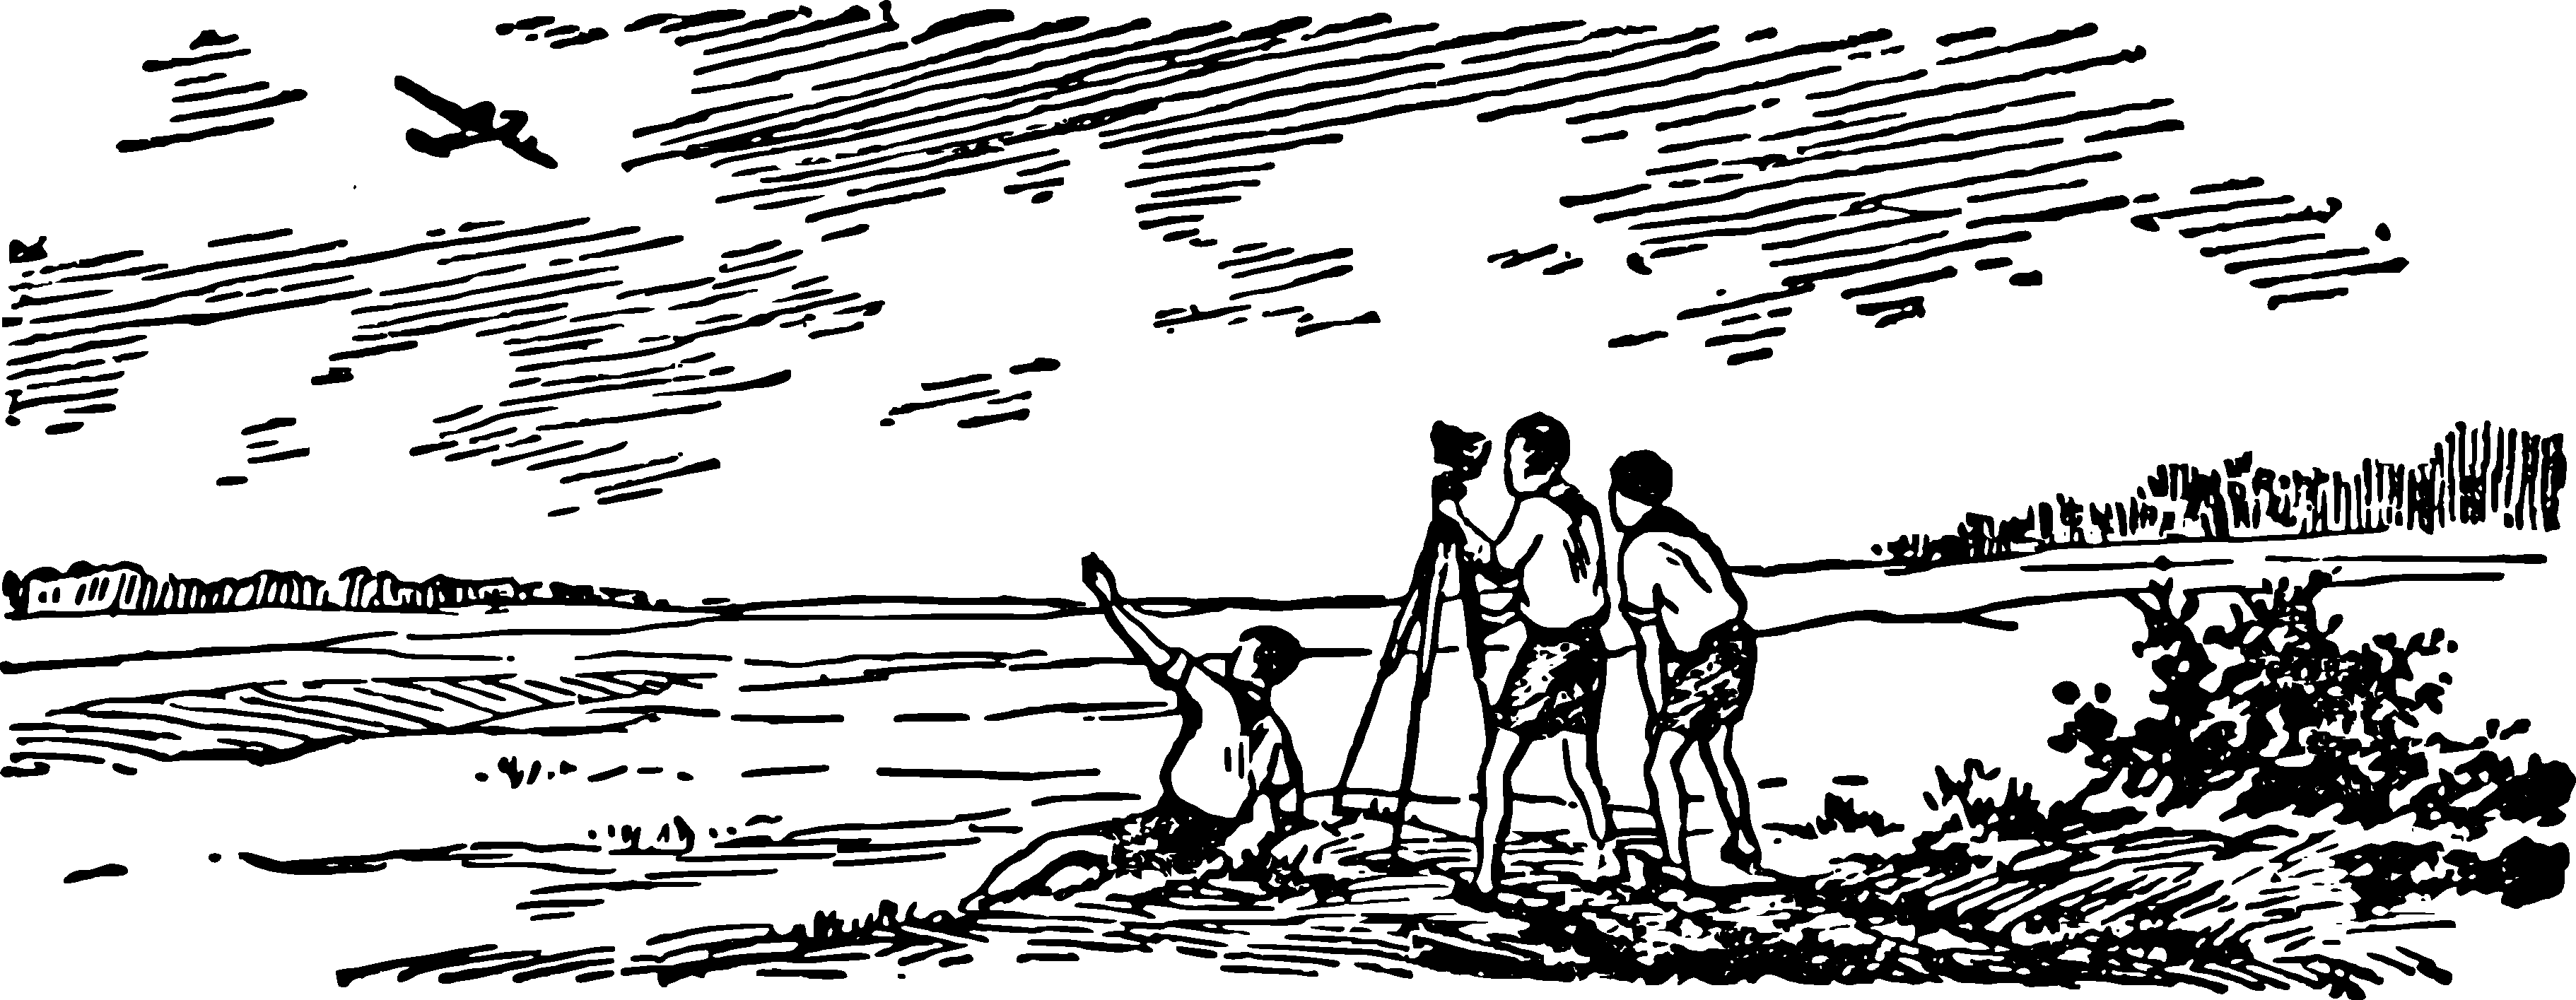
\includegraphics[width=1.2\textwidth]{figures/ch-03/fig-ch-03-head.pdf}\bigskip}

\chapter{Geometry In The Open Field}
\label{ch-03}

\section{Visible sizes of the Moon}
\label{sec-3.1}


What size does the full moon in the sky seem to you? Different people give quite different answers to this question.

Estimates like ``the size of a plate,'' ``the size of an apple,'' ``the size of a human face,'' and so on, are extremely vague, indefinite, indicating only that those answering do not understand the essence of the question.

The correct answer to such an apparently ordinary question can only be given by someone who clearly understands what exactly needs to be understood by the ``apparent'' or ``visible'' size of an object. Few suspect that here we are referring to the magnitude of a certain angle -- precisely the angle formed by two straight lines drawn to our eye from the extreme points of the object under consideration; this angle is called the ``angle of view'' or ``angular size of the object'' (\figr{fig-061}). 

\begin{figure}[h!]
\centering
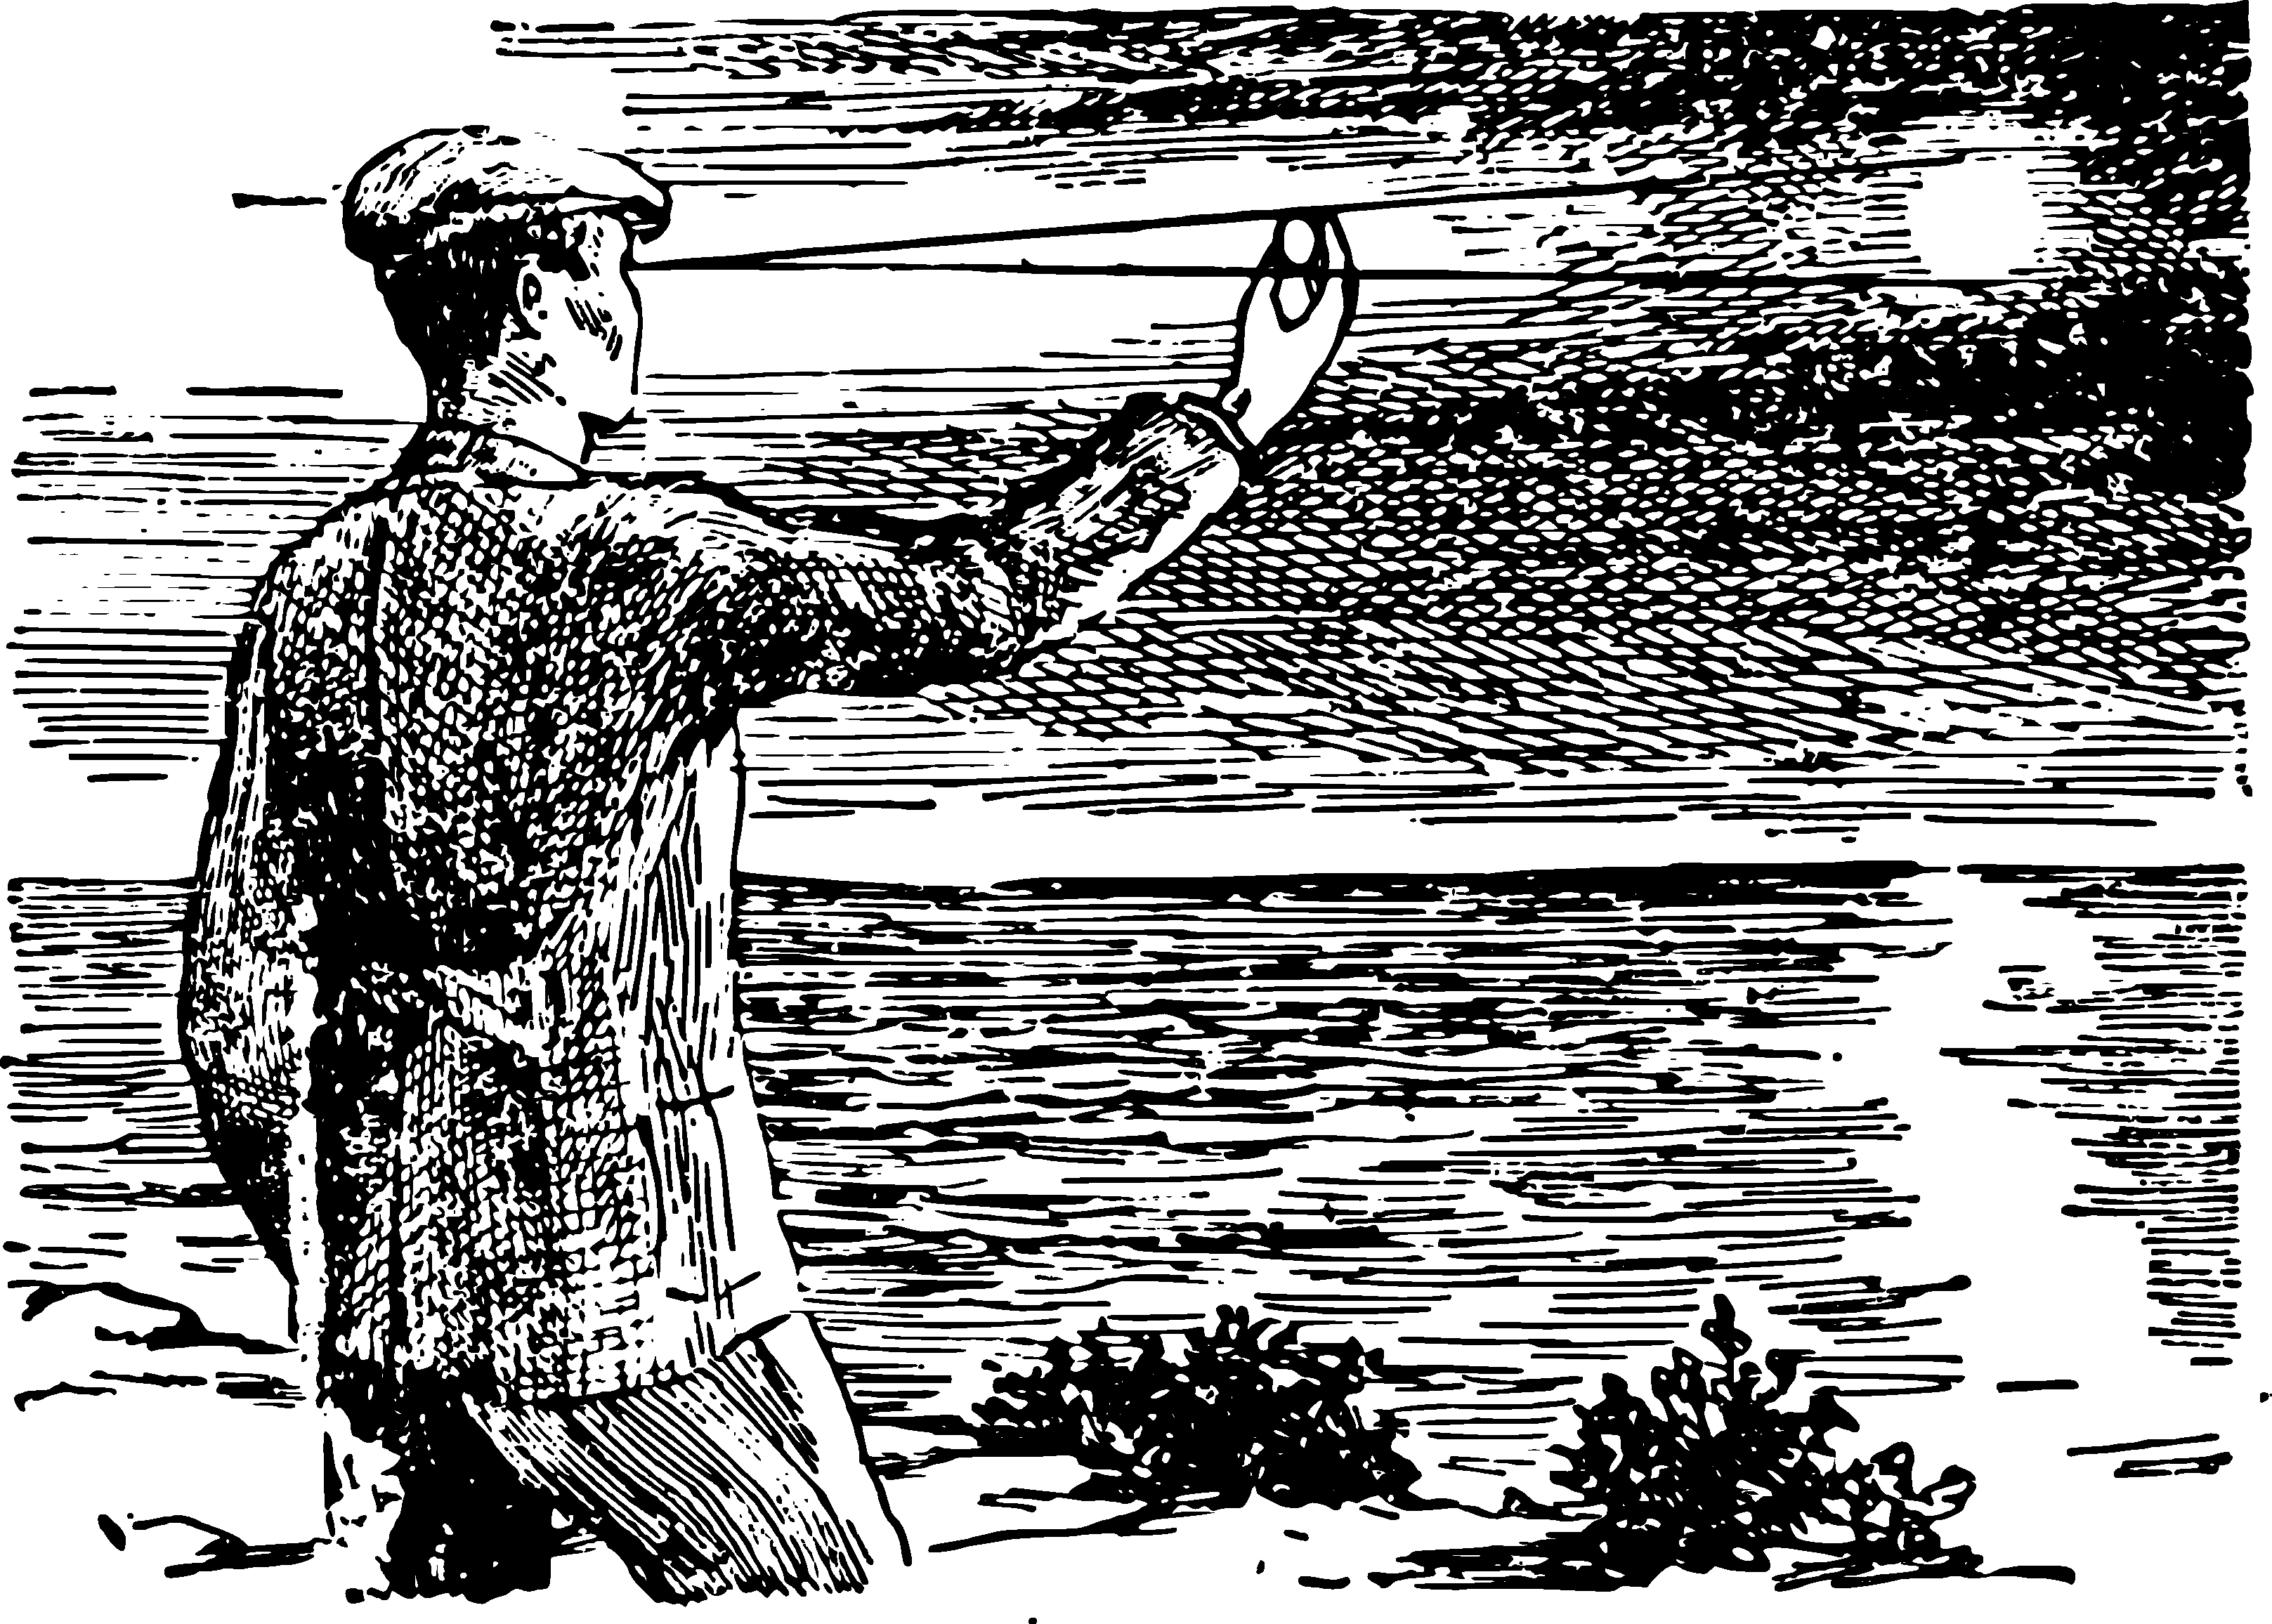
\includegraphics[width=0.9\textwidth]{figures/ch-03/fig-061.pdf}
\sidecaption{What is the angle of view or angular size of the object.\label{fig-061}}
\end{figure}

And when the apparent size of the Moon in the sky is assessed by comparing it with the sizes of a plate, an apple, and so forth, such answers are either completely meaningless or should imply that the Moon is visible in the sky at the same angle as the plate or apple. But such an indication alone is still insufficient: after all, we see a plate or an apple under different angles depending on their distance: up close -- under larger angles, far away -- under smaller ones. To introduce clarity, it is necessary to specify from what distance the plate or apple is being observed. Comparing the sizes of distant objects with the sizes of others, the distance of which is not indicated, is a very common literary technique employed by even first-rate writers. It creates a certain impression due to its closeness to the familiar psychology of most people, but it does not produce a clear image\ldots{} Here's an example from Shakespeare's \emph{King Lear}; it describes (by Edgar) the view from a high cliff by the sea:
\begin{quote}
\emph{How terrifying! How my head spins!\\
How low to cast my gaze\ldots{}\\
The rooks and crows that flutter there in the air at mid-distance,\\ Seem barely as large as flies. Halfway down Hangs a man gathering seaweed\dots{} \\
What a dreadful trade! He seems to me no bigger than his head.\\
The fishermen walking along the shore -- like mice;\\
and that tall ship at anchor has shrunk to the size of its boat;\\ its boat -- a floating dot, As if too small for sight\dots{}}
\end{quote}
These comparisons would provide a clear idea of distance if accompanied by indications of the degree of remoteness of the objects being compared (mice, the human head, crows, boat \dots{}). Similarly, when comparing the size of the moon with that of a plate or apples, indications of how far these everyday objects should be from the eye are necessary.

This distance turns out to be much greater than commonly thought. Holding an apple at arm's length, you not only obscure the Moon but also a significant portion of the sky. Suspend the apple on a string and gradually move away from it until it just covers the full lunar disk: in this position, the apple and the Moon will have the same apparent size for you. By measuring the distance from your eye to the apple, you will find that it is approximately 10 meters. This is how far you would need to move the apple away from you for it to truly seem to be the same size as the Moon in the sky! A plate, on the other hand, would need to be moved about 80 meters away from you, or about fifty steps.

What is said may seem unbelievable to anyone hearing it for the first time; however, it is indisputable and follows from the fact that we perceive the Moon at an angle of only \emph{half a degree}. We rarely have to estimate angles in our everyday lives, and therefore most people have a very vague idea of the magnitude of an angle with a small number of degrees, such as an angle of \ang{1}, \ang{29}, or \ang{59} (not to mention surveyors, draftsmen, and other specialists accustomed to practically measuring angles). We only estimate large angles more or less reasonably, especially if we manage to compare them with angles familiar to us between the hands of a clock; everyone, of course, is familiar with angles of \ang{90}, \ang{60}, \ang{30}, \ang{120}, \ang{150}, which we are so accustomed to seeing on a dial (at 8 o'clock, 2 o'clock, 1 o'clock, 4 o'clock, 5 o'clock) that even without distinguishing the numbers, we guess the time based on the size of the angle between the hands. But we usually see small and individual objects at much smaller angles and therefore completely lack the ability to even approximately estimate angles of view.


\section{Angle of View}
\label{sec-3.2}

To provide a concrete example of a one-degree angle, let's calculate how far an average-height person (1.7 meters) should move away from us to appear at such an angle. Translating the problem into the language of geometry, let's say we need to calculate the radius of a circle, the arc of which at \ang{1} has a length of 1.7 meters (strictly speaking, not an arc, but a chord, but for small angles, the difference between the lengths of the arc and the chord is negligible). We reason as follows: if the arc at \ang{1} equals 1.7 meters, then the full circumference containing \ang{360} will have a length of $1.7 \times 360 = \SI{610}{\meter}$, and the radius will be $1/2\pi$ the length of the circumference; if we take the value of $\pi$ as approximately 22/7, then the radius will be equal to
\begin{equation*}%
 \frac{610}{44/7} \approx \SI{98}{\meter}.
\end{equation*}
\begin{figure}[h!]
\centering
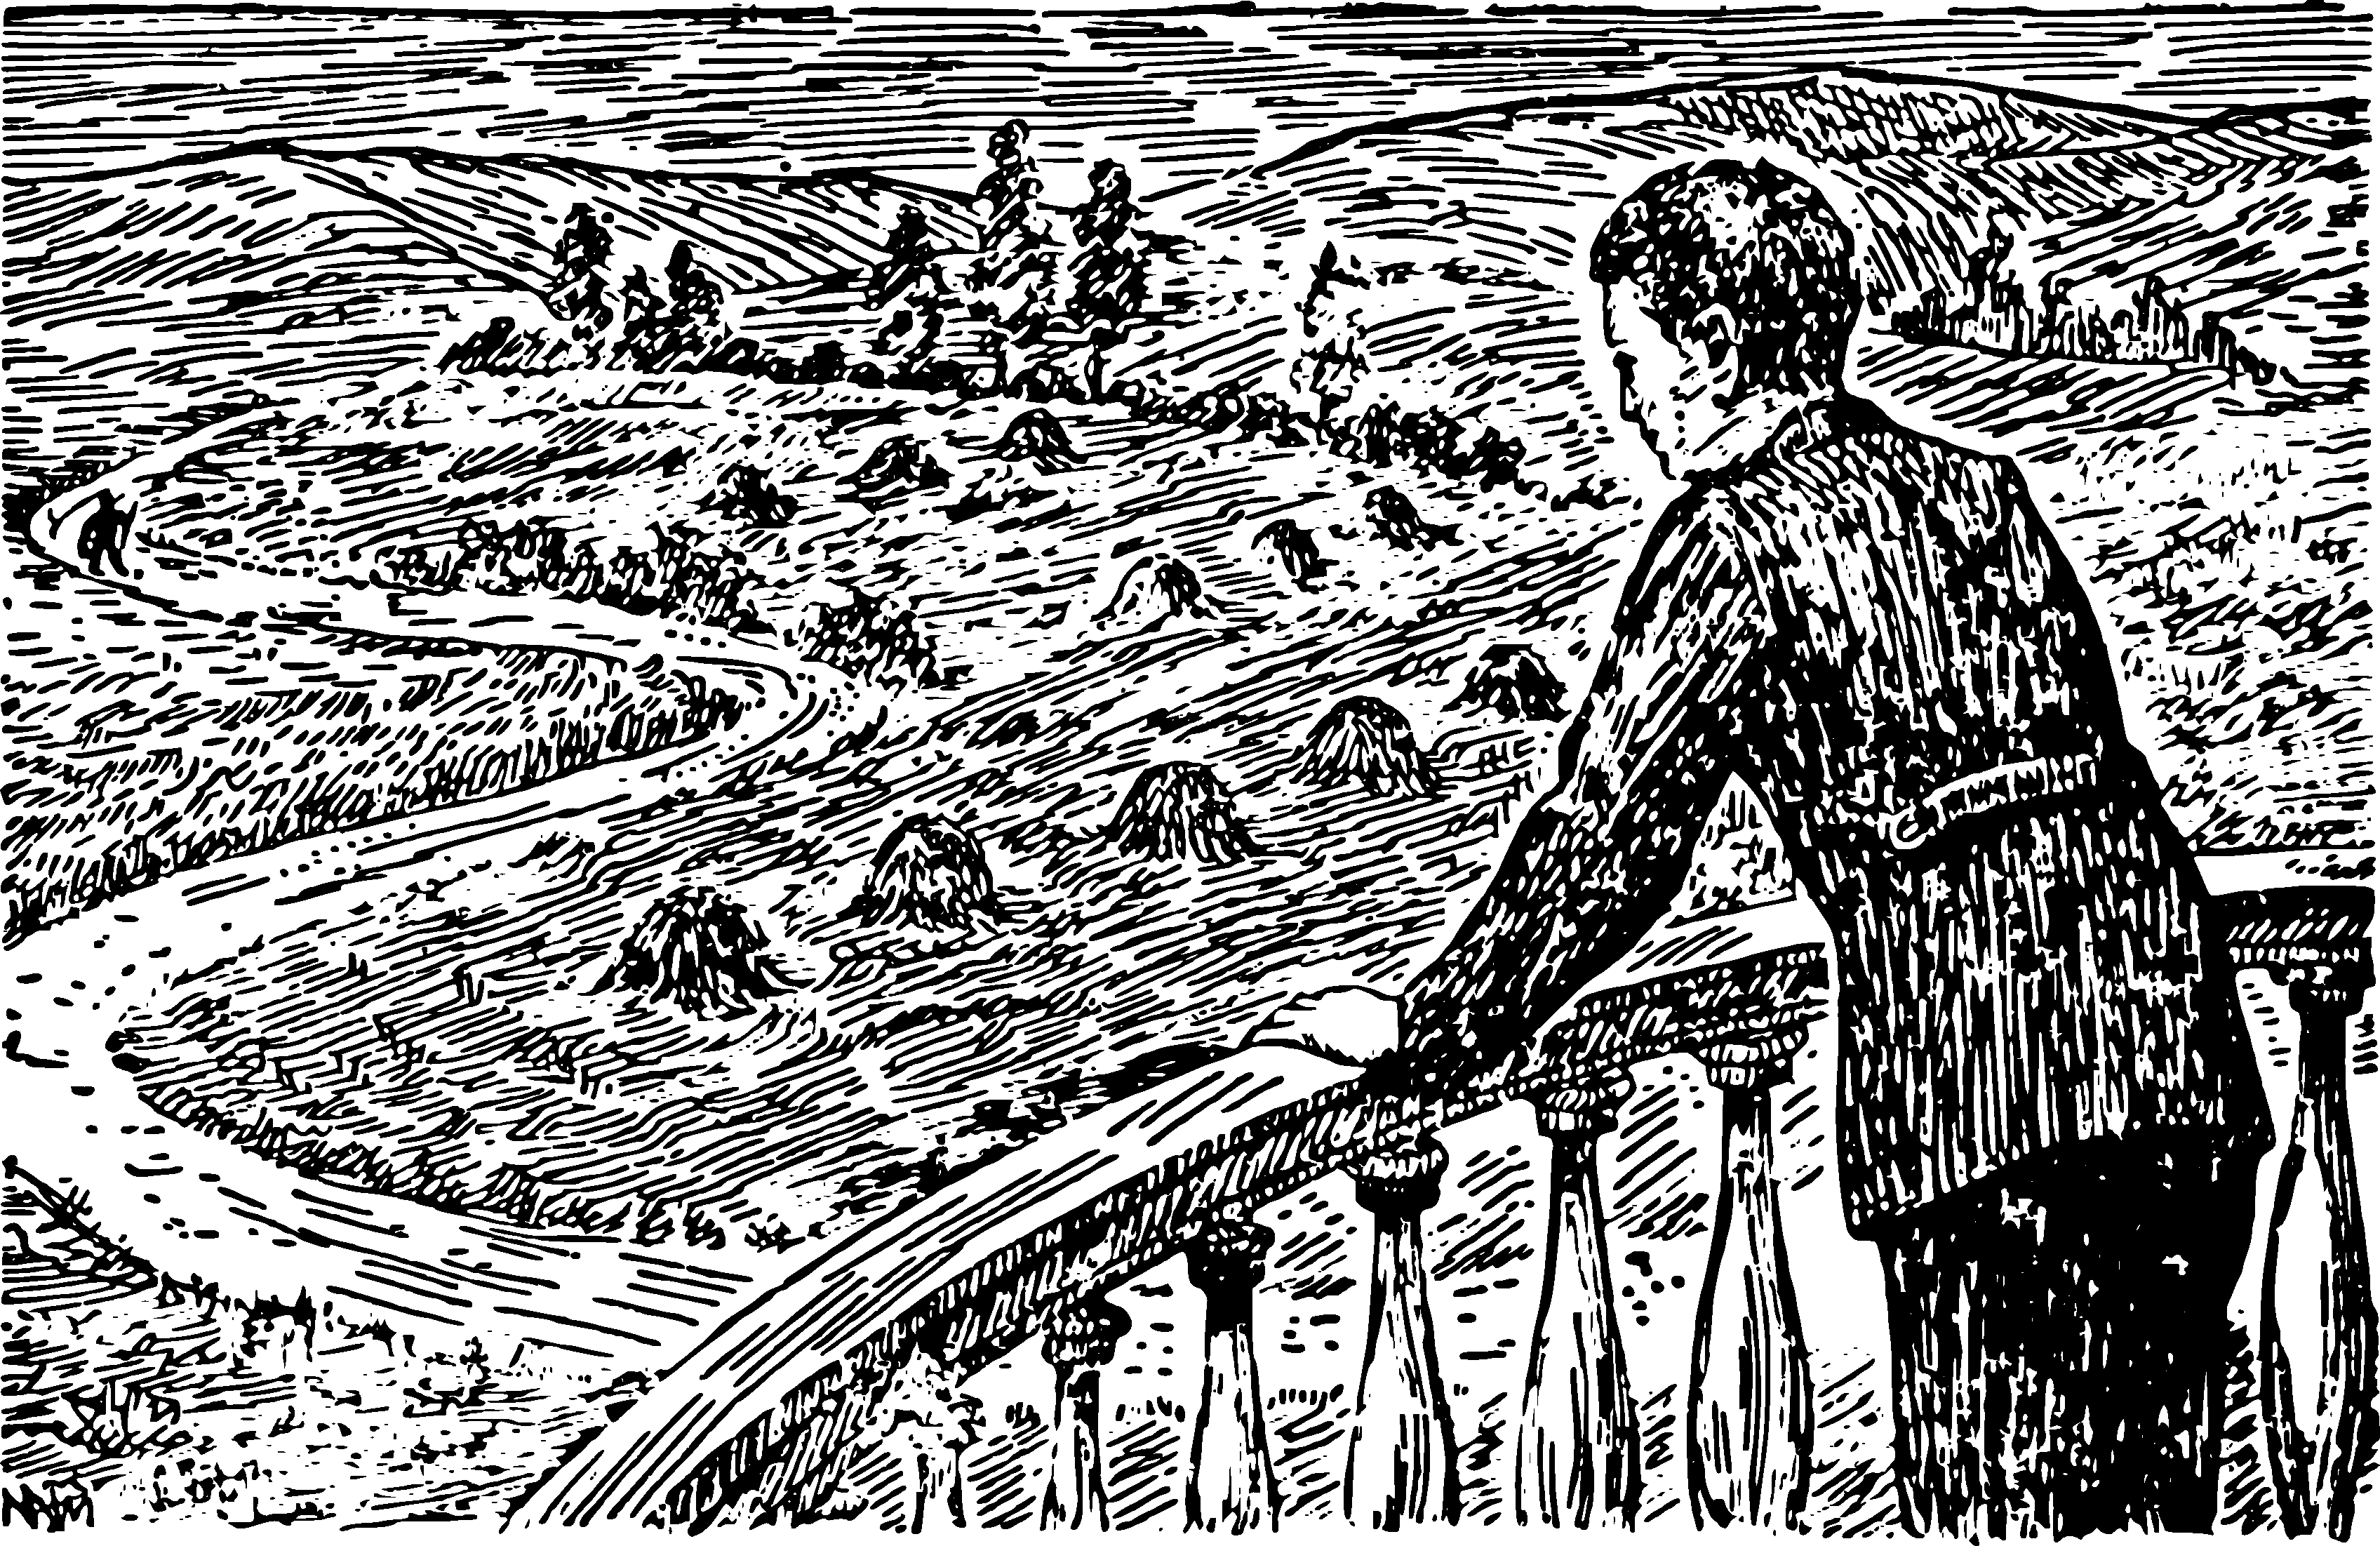
\includegraphics[width=0.9\textwidth]{figures/ch-03/fig-062.pdf}
\sidecaption{The human figure is visible from a distance of about hundred meters at an angle of \ang{1}.\label{fig-062}}
\end{figure}
So, a person appears at an angle of \ang{1} if they are approximately at a distance of 100 meters from us (\figr{fig-062}). If they move twice as far away -- to 200 meters -- they will be seen at an angle of half a degree; if they approach to a distance of 50 meters, the angle of view will increase to \ang{2}, and so on. It is also easy to calculate that a stick of 1 meter in length should appear to us at an angle of 1° at a distance of $360/(44/7) = \SI{57}{\meter}$.

At the same angle, we perceive an object of 1 cm from a distance of 57 cm, 1 km from a distance of 57 km, and so on -- in general, any object from a distance 57 times greater than its diameter. If we remember this number -- 57, we can quickly and easily perform all calculations related to the angular size of an object. For example, if we want to determine how far we need to move an apple with a diameter of 9 cm to see it at an angle of \ang{1}, it is sufficient to multiply 9 by 57 -- we get 513 cm, or about 5 meters; from twice the distance, it is perceived at half the angle -- half a degree, i.e., it appears the size of the Moon.

In the same way, for any object, we can calculate the distance at which it appears to be the same size as the lunar disk.

\section{Plate and Moon} 
\label{sec-3.3}

\ques At what distance should a plate with a diameter of 25 cm be moved away to appear the same size as the Moon in the sky?

\ans $\SI{25}{\centi\meter} \times 57 \times 2 = \SI{2850}{\centi\meter} = \SI{28}{\meter}$.

\section{Moon and Copper Coins} 
\label{sec-3.4}

\ques Perform the same calculation for a five-kopeck coin (diameter 25 mm) and a three-kopeck coin (22 mm).

\ans For the five-kopeck coin: \(0.025 \text{ m} \times 57 \times 2 = 2.85 \text{ meters}\),
For the three-kopeck coin: \(0.022 \text{ m} \times 57 \times 2 = 2.514 \text{ meters}\).

If it seems unbelievable to you that the Moon appears no larger than a two-kopeck coin from a distance of four steps or an ordinary pencil from a distance of 80 cm, -- hold the pencil at arm's length against the full Moon disk: it will easily cover it. Strangely enough, the most suitable comparison object for the Moon in terms of perceived size is not a plate, not an apple, not even a cherry, but a pea or, even better, a match head! Comparing it to a plate or an apple implies moving them to an unusually large distance; we see an apple in our hands or a plate on the dining table ten to twenty times larger than the lunar disk. And only a match head, which we examine at a distance of 25 cm from the eye (`distance of distinct vision'), is seen at an angle of half a degree, i.e., the same size as the Moon.

The fact that the lunar disk deceptively appears to grow in the eyes of most people by 10 to 20 times is one of the most curious optical illusions. It depends, one might think, mostly on the \emph{brightness} of the Moon: the full moon stands out against the sky much more sharply than plates, apples, coins, and other comparison objects do amidst the surrounding environment.\sidenote{For the same reason, the incandescent filament of an electric light bulb seems to us much thicker than in a cold, non-luminous state.}

This illusion is imposed on us with such irresistible force that even artists, distinguished by a keen eye, succumb to it alongside others and depict the full moon in their paintings much larger than it should be. It is enough to compare the landscape painted by an artist with a photograph to be convinced of this.

The same applies to the Sun, which we see from Earth at the same angle of half a degree; although the true diameter of the solar sphere is 400 times larger than that of the lunar one, its distance from us is also 400 times greater.


\section{Sensational Photographs}
\label{sec-3.5}

To explain the important concept of the angle of view, let's deviate a bit from our main topic — geometry in open fields — and provide a few examples from the realm of photography.

On the movie screen, you've surely seen such catastrophes as train collisions or such incredible scenes as a car driving on water.

Recall the movie `Captain Grant's Children.' What a strong impression -- isn't it? -- the scenes of the shipwreck during the storm or the sight of crocodiles surrounding the boy stuck in the swamp left on you. Of course, no one thinks that such photographs were taken directly from real life. But how were they obtained?
\begin{figure}[h!]
\centering
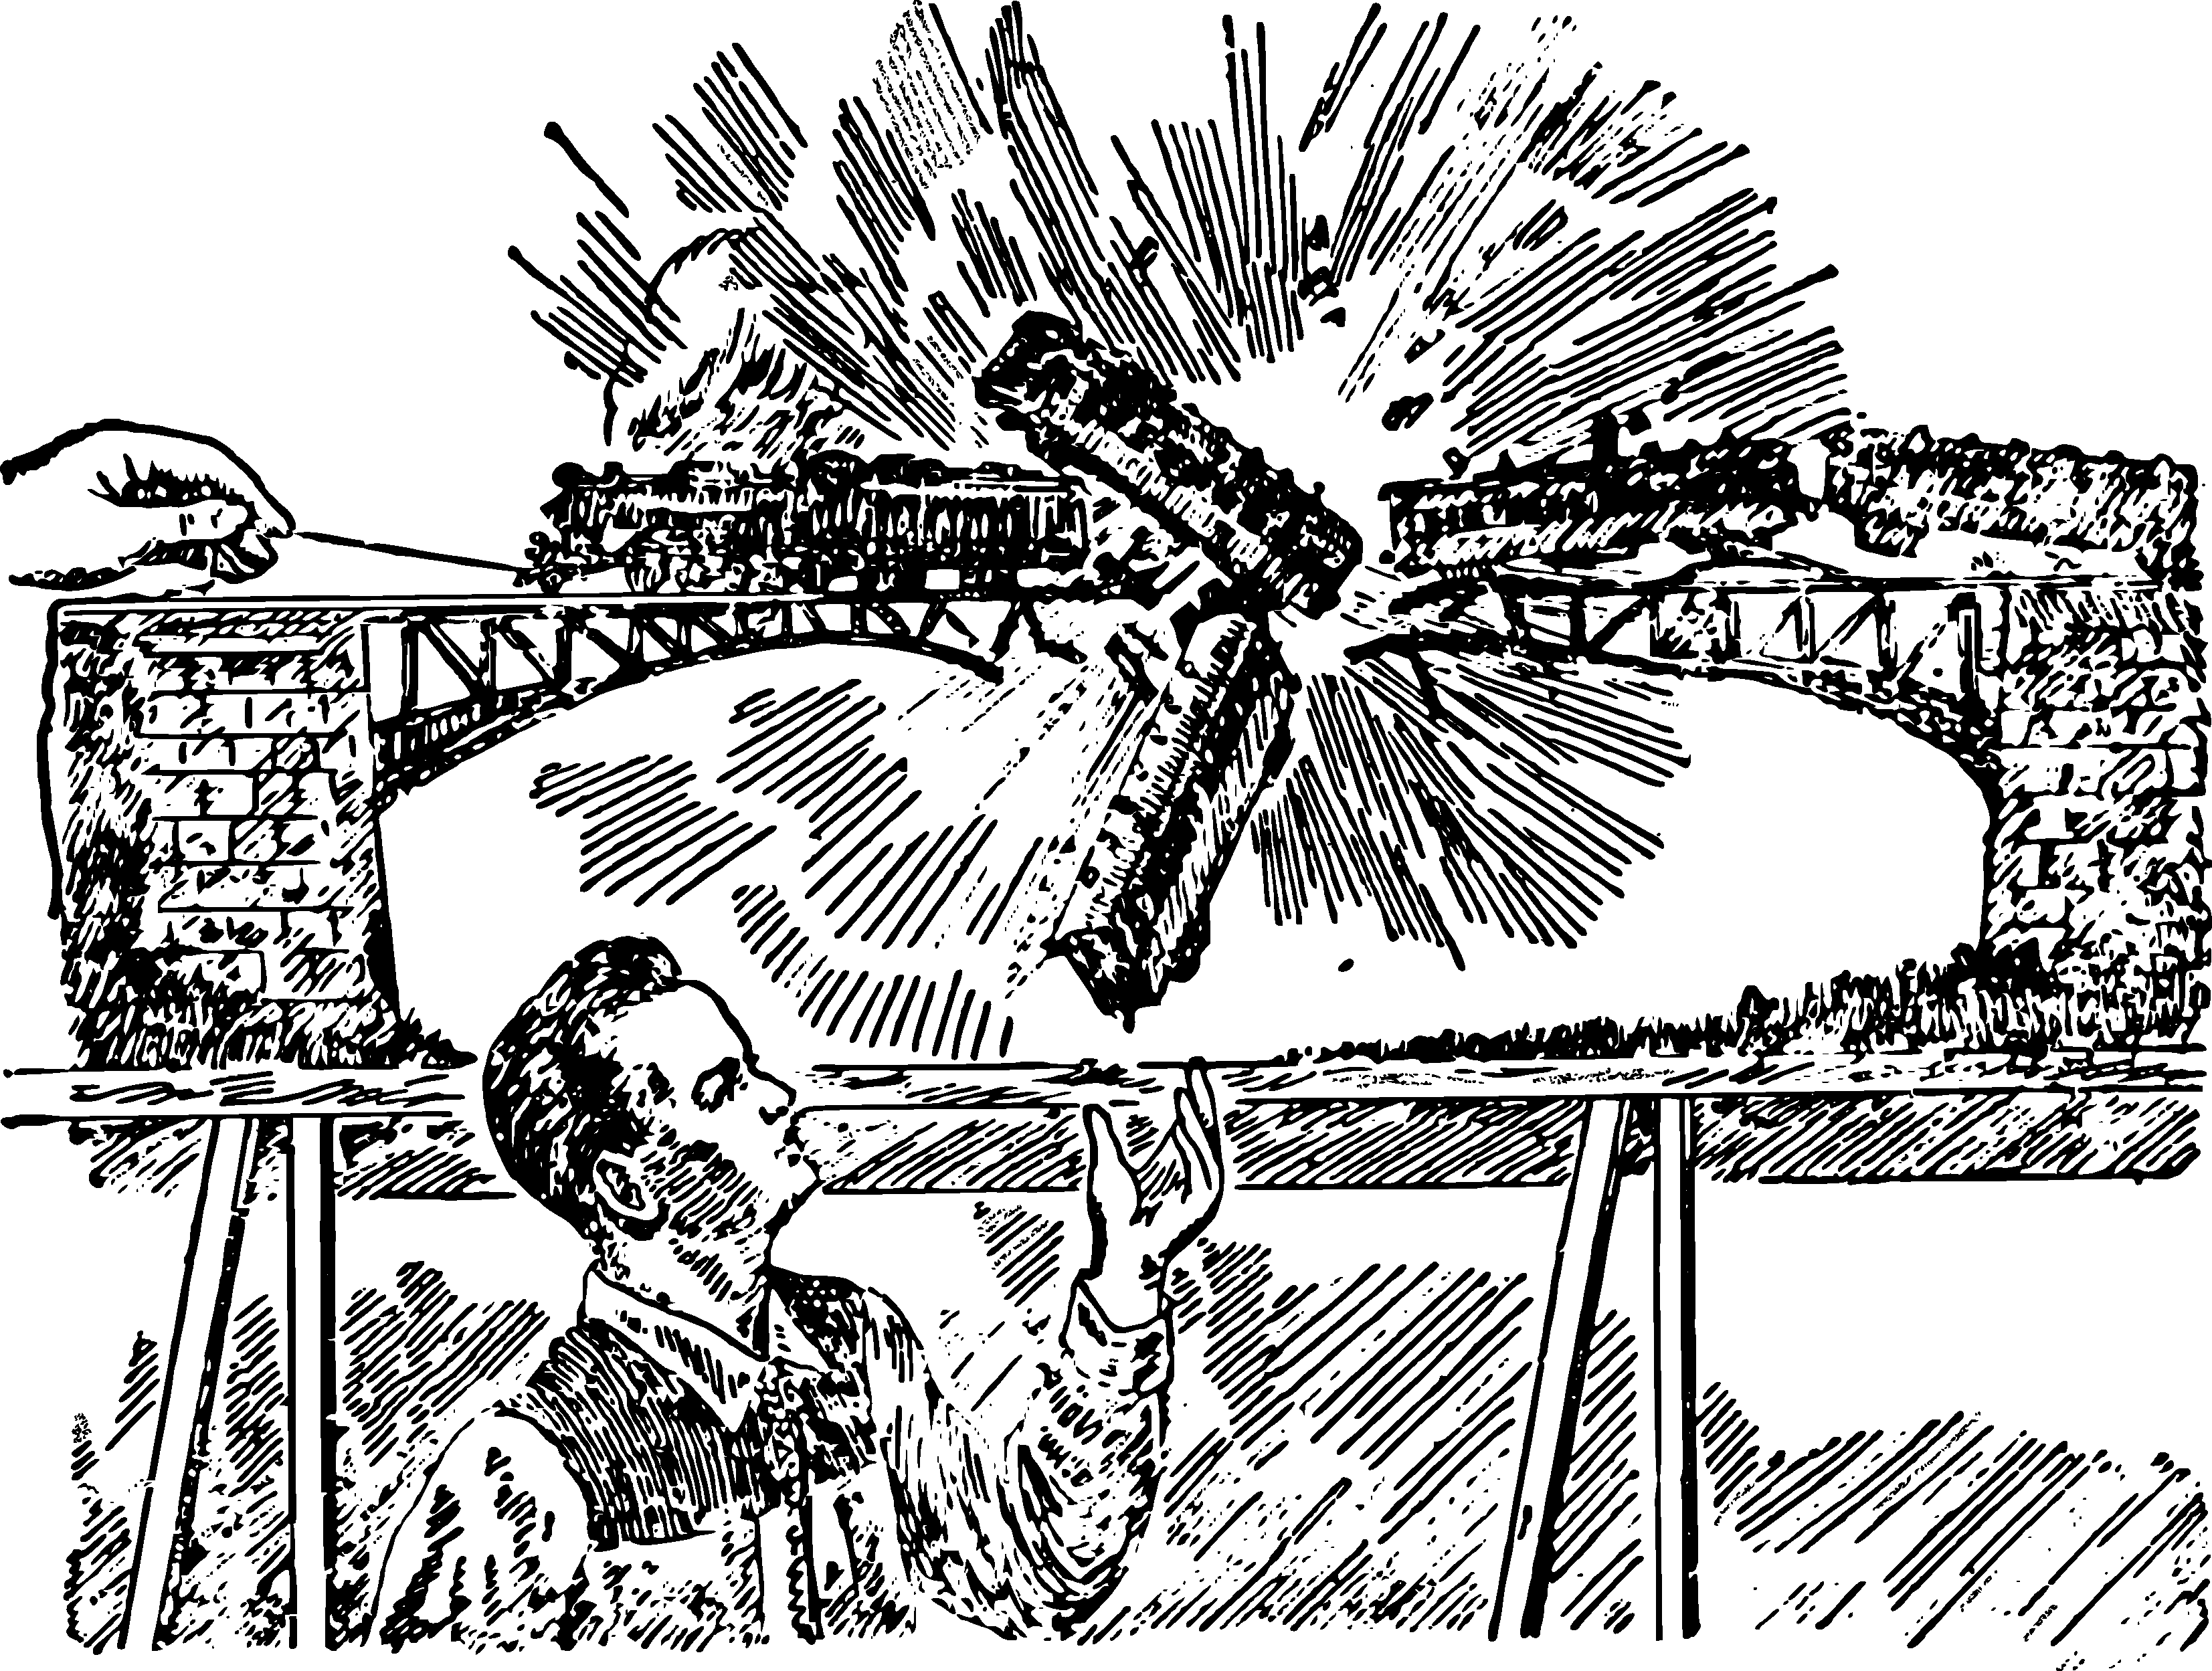
\includegraphics[width=0.9\textwidth]{figures/ch-03/fig-063.pdf}
\sidecaption{Preparing a train accident for filming.\label{fig-063}}
\end{figure}


The secret is revealed by the illustrations attached here. In \figr{fig-063}, you see the `catastrophe' of a toy train in a toy setting; in \figr{fig-064} -- a toy car being pulled on a string behind an aquarium. This is the `nature' from which the film was shot. But why do we succumb to the illusion when we see these images on the screen, as if we were looking at real trains and cars? After all, here, in the illustrations, we would immediately notice their miniature size, even if we couldn't compare them with the size of other objects. The reason is simple: toy trains and cars are filmed for the screen from a very close distance; therefore, they appear to the viewer at approximately the same angle of view as we usually see real trains and cars. That's the whole secret of the illusion.

\begin{figure}[h!]
\centering
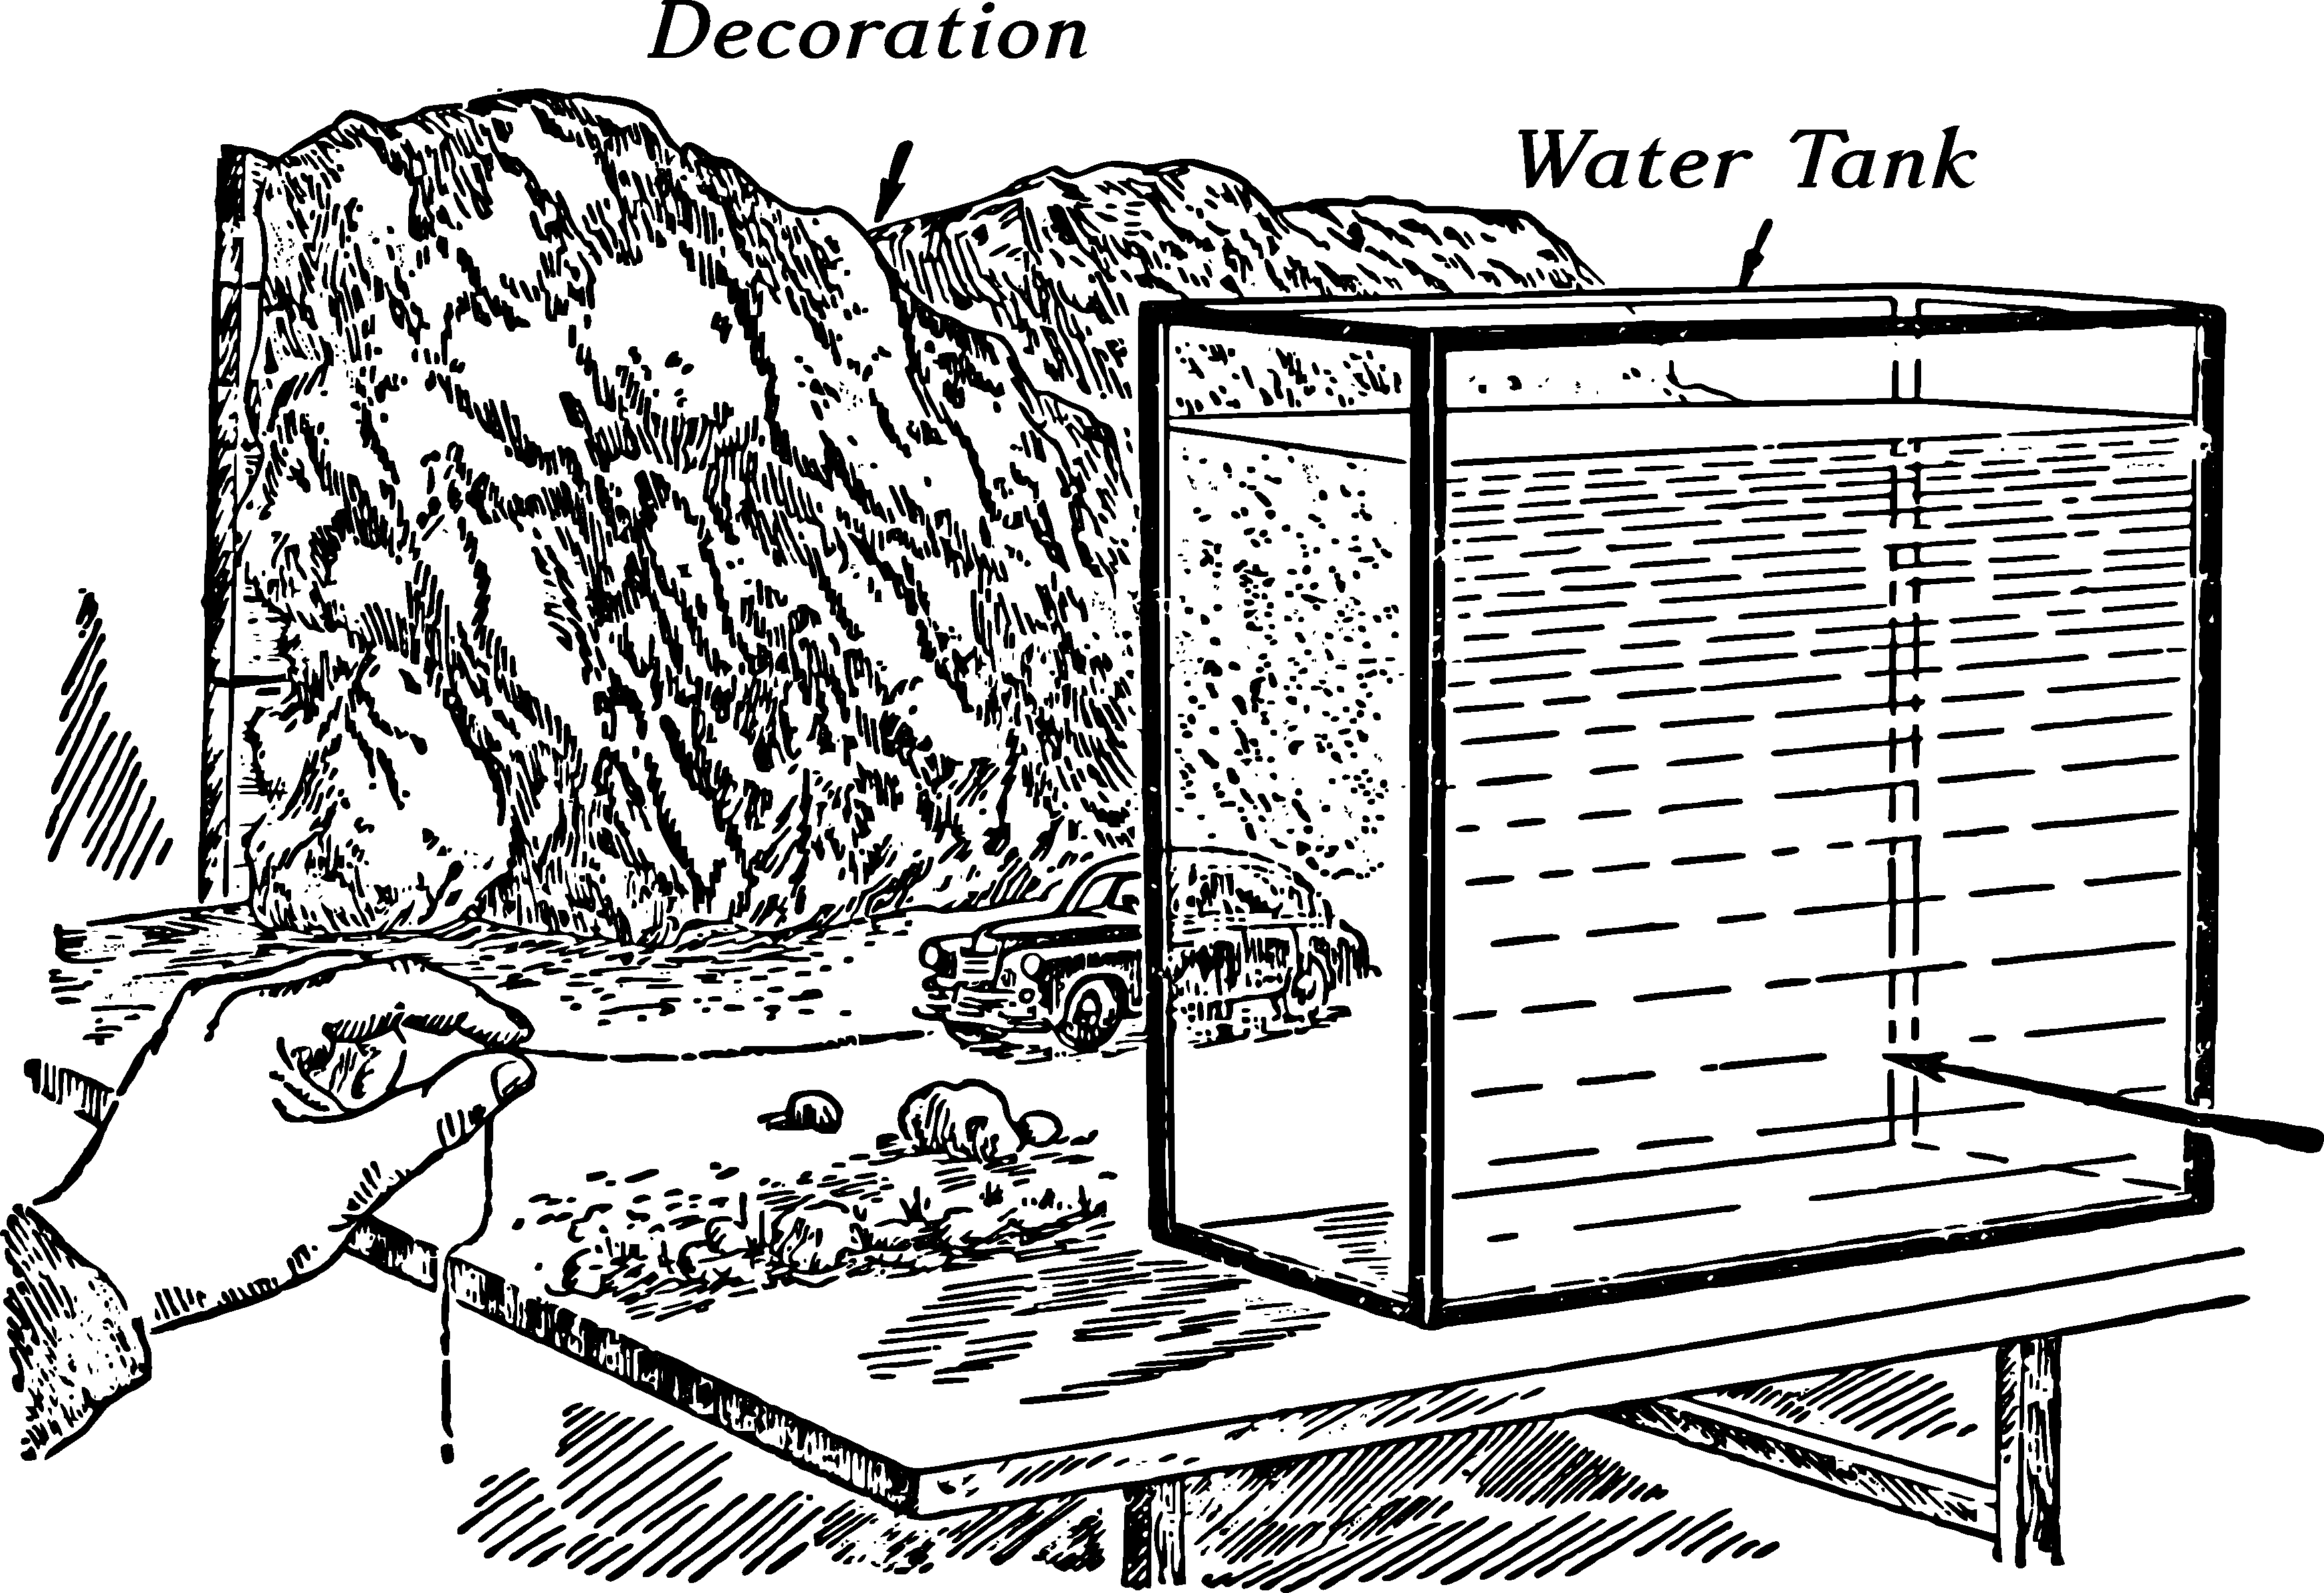
\includegraphics[width=0.9\textwidth]{figures/ch-03/fig-064.pdf}
\sidecaption{The underwater road trip.\label{fig-064}}
\end{figure}

Or here's another frame from the movie `Ruslan and Ludmila' (\figr{fig-065}). A huge head and a small Ruslan on a horse. The head is placed on a model field close to the camera. And Ruslan on the horse -- at a considerable distance. That's the entire secret of the illusion.

\begin{figure}[h!]
\centering
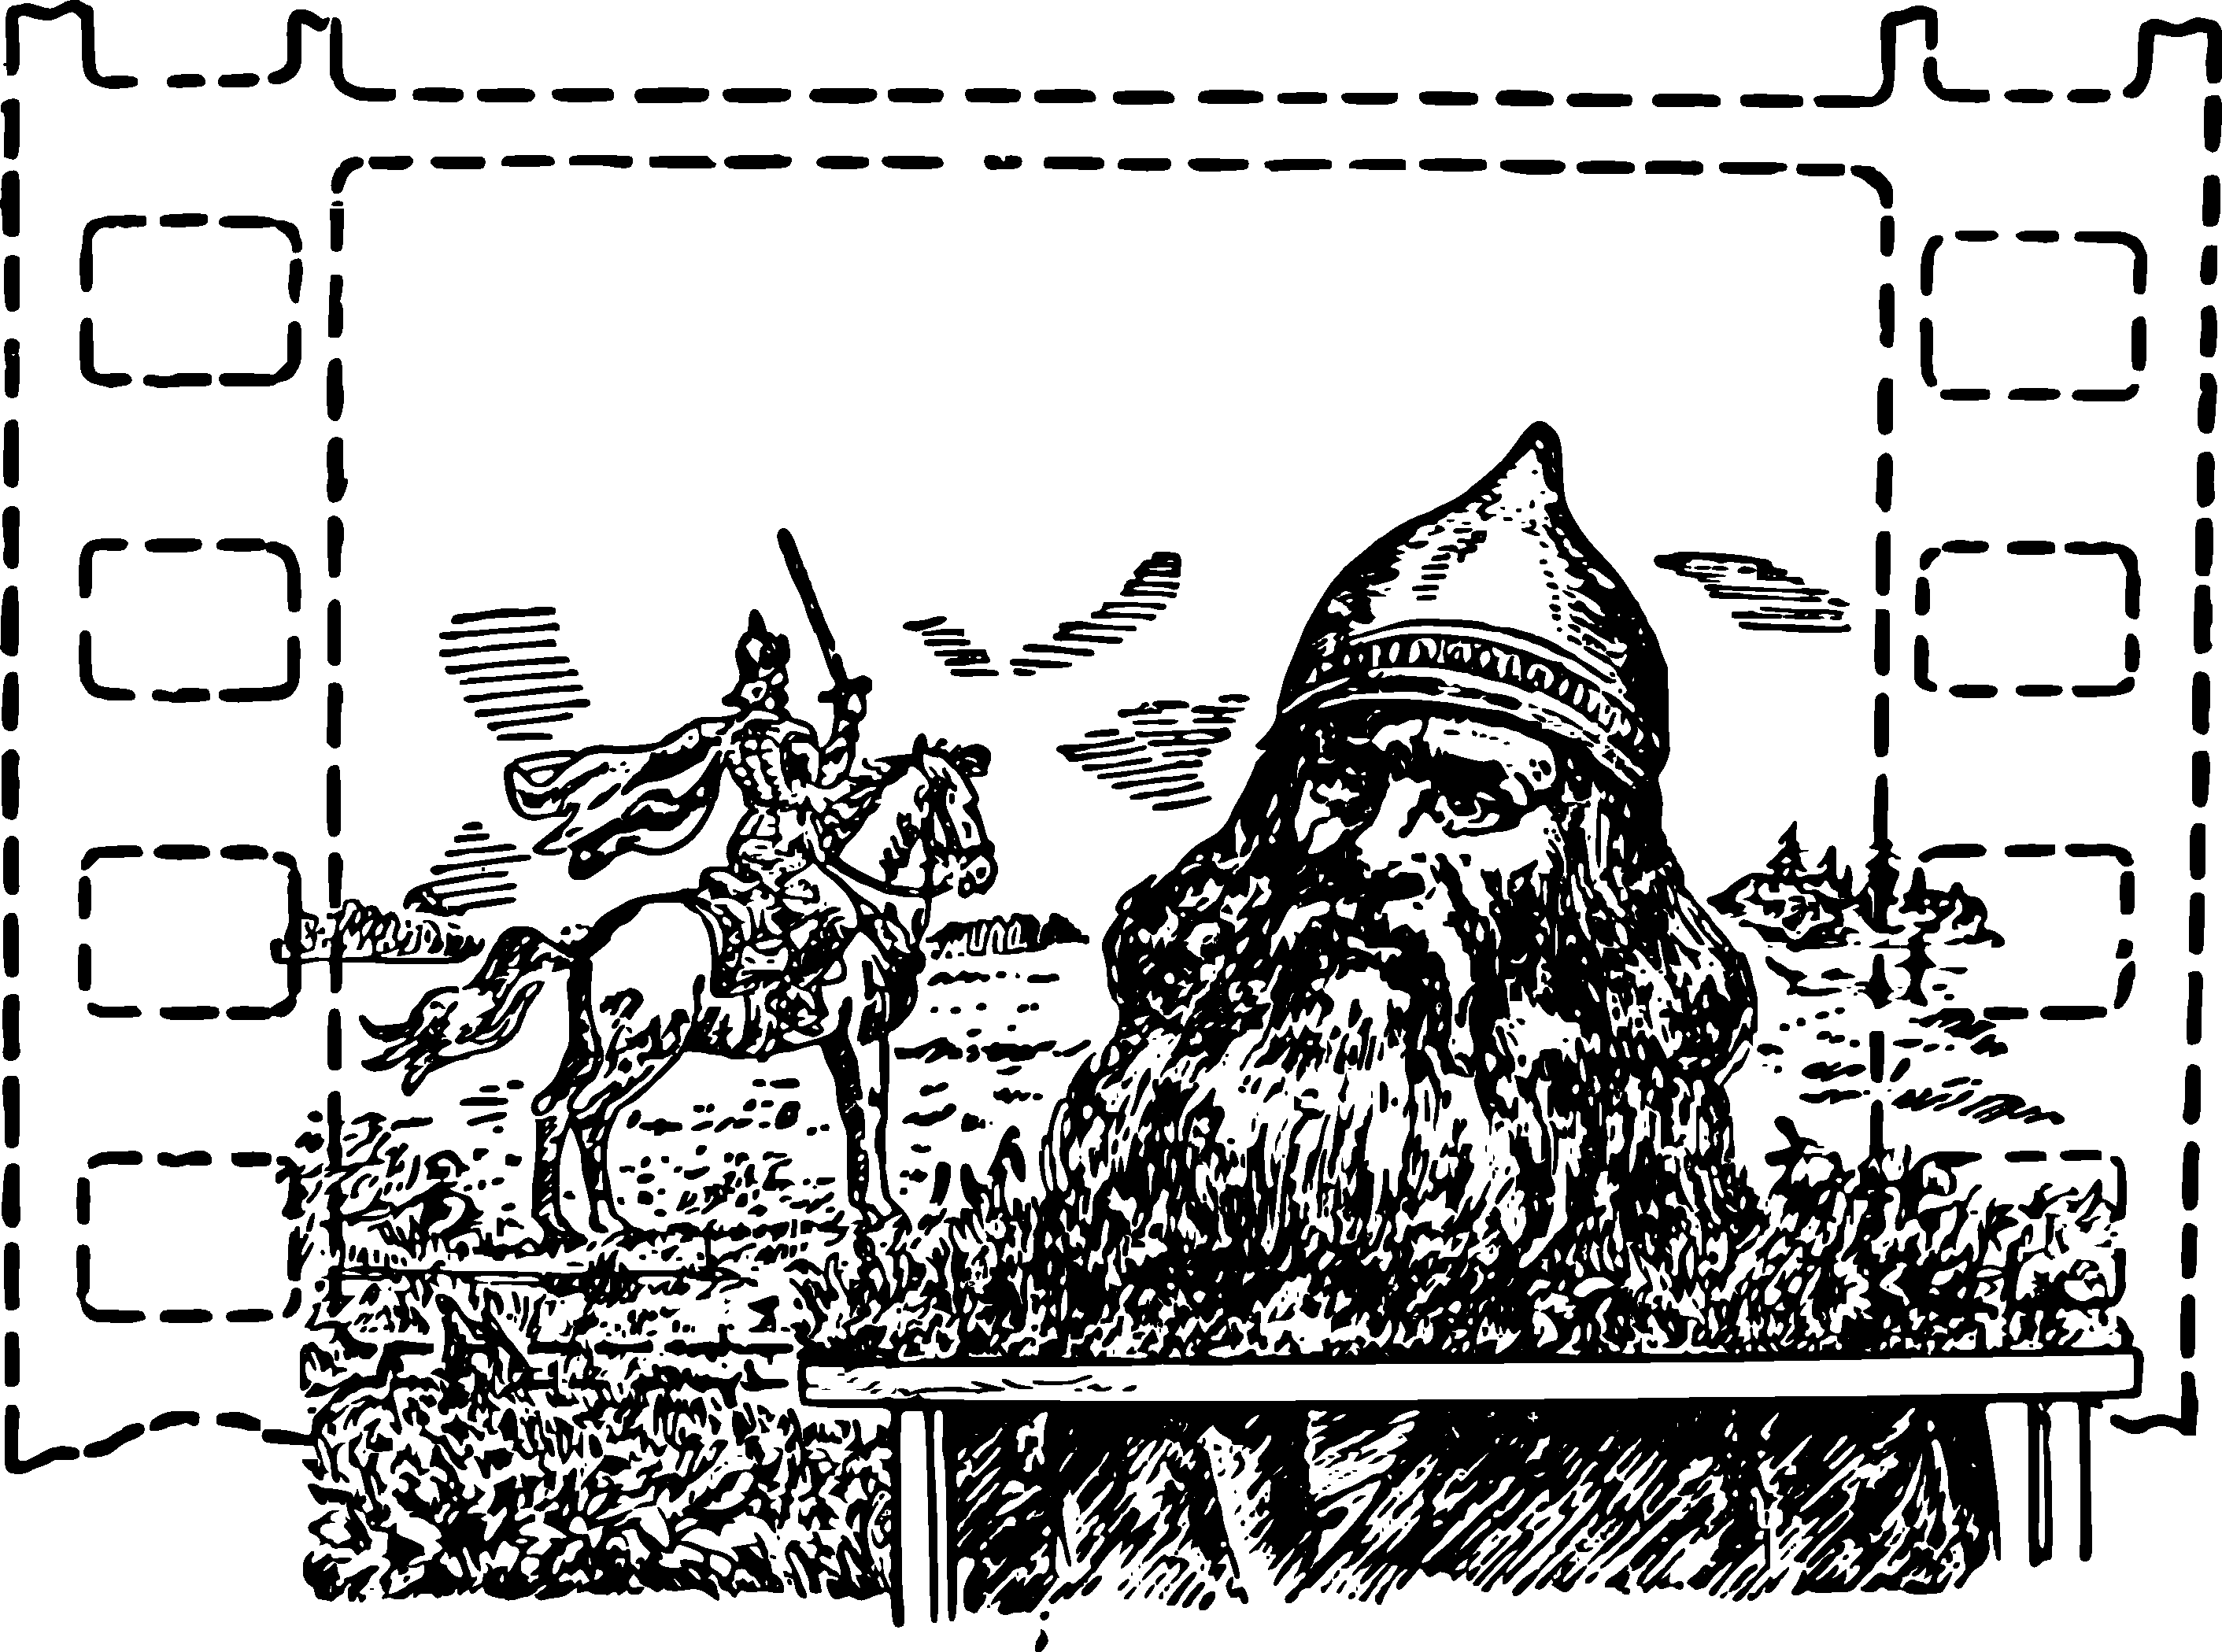
\includegraphics[width=0.9\textwidth]{figures/ch-03/fig-065.pdf}
\sidecaption{A shot from the movie \emph{Ruslan and Lyudmila}.\label{fig-065}}
\end{figure}

\section{Reservoir Set Decoration}
\label{sec-3.6}

\figr{fig-066} is another example of an illusion based on the same principle. You see a strange landscape reminiscent of the nature of ancient geological epochs: bizarre trees resembling giant mosses, on them -- huge water drops, and in the foreground -- a gigantic monster resembling harmless frogs. Despite such an unusual view, the drawing is made with subtlety: it's nothing but a small patch of soil in the forest, only drawn from an unusual angle of view. We never see moss stems, water drops, frogs, etc., at such a large angle of view, and therefore the drawing seems so alien, unfamiliar to us. Before us is a landscape as we would see it if we were shrunk to the size of an ant. 

\begin{marginfigure}[-1cm]%[h!]
\centering
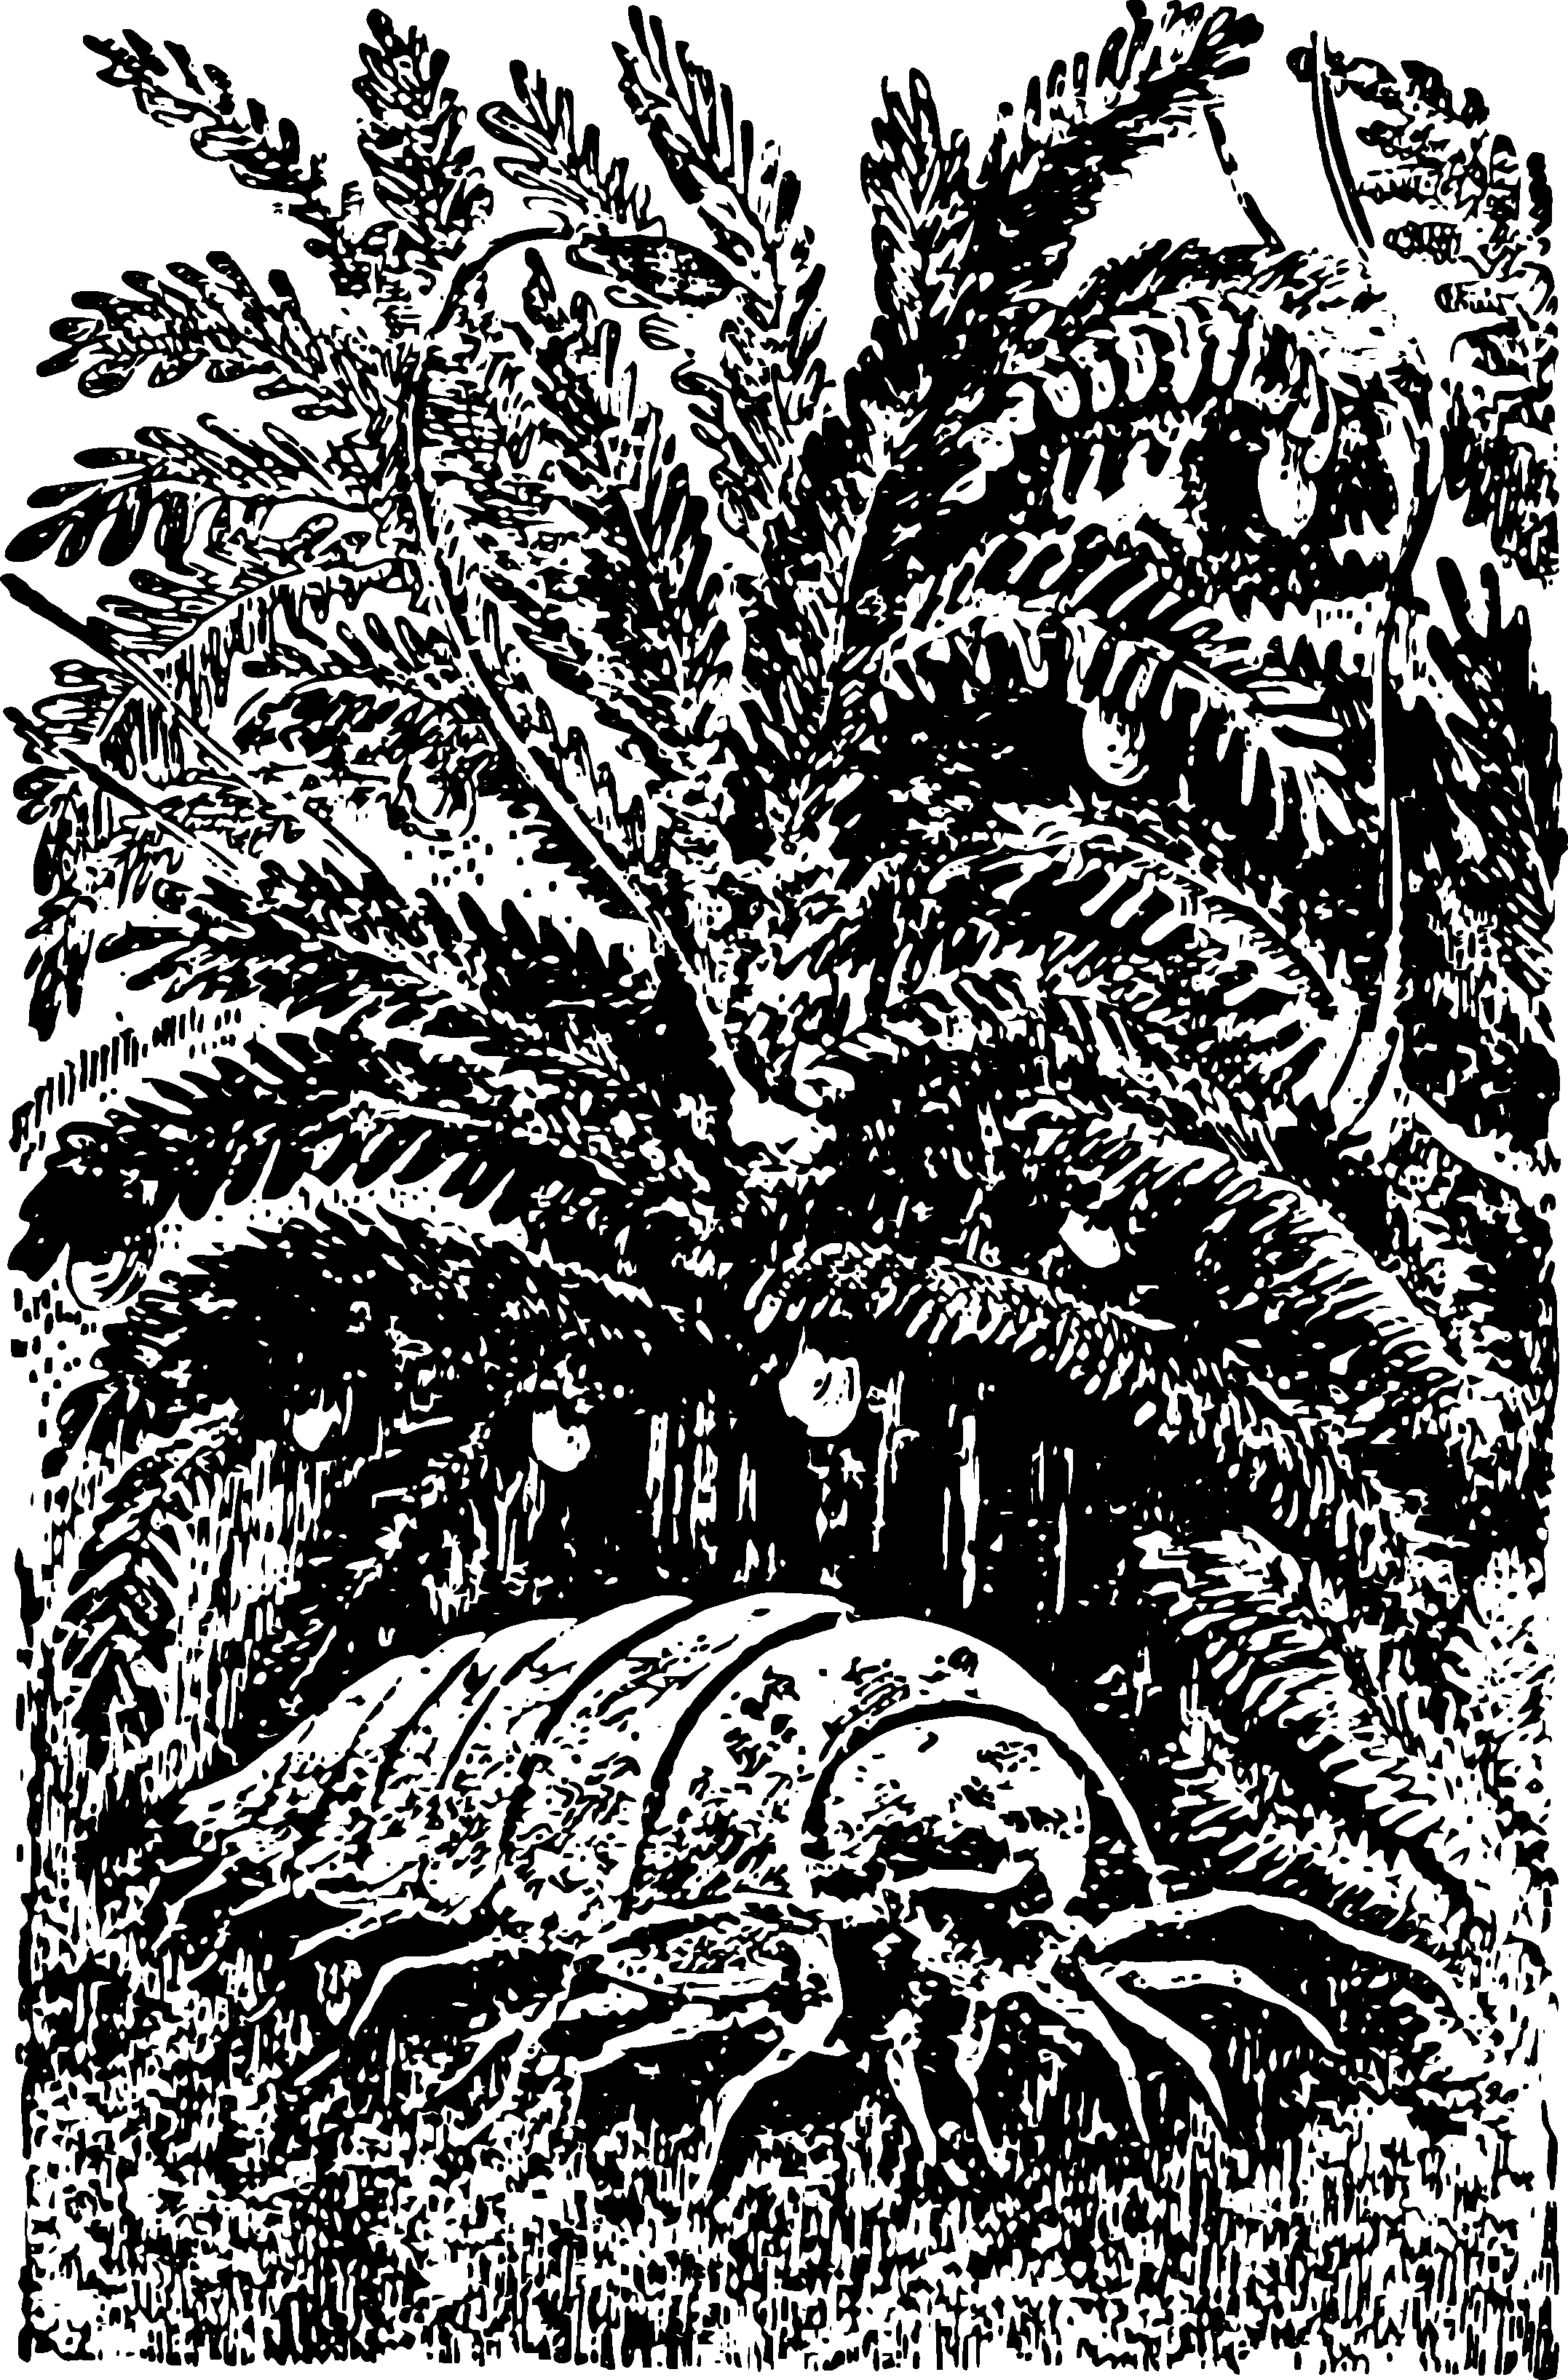
\includegraphics[width=\textwidth]{figures/ch-03/fig-066.pdf}
\sidecaption{Mysterious landscape depicted from nature.\label{fig-066}}
\end{marginfigure}

Swindlers from bourgeois newspapers act in the same way to create fake reportage photographs. One foreign newspaper once published a note criticising the city administration for allowing huge snow mountains to form on the city streets. To support this, an impressive photo of one such mountain was provided (\figr{fig-067}, left). Upon examination, it turned out that the nature for the photograph was a small snowdrift, taken by the `joker' photographer from a very close distance, i.e., at an unusually large angle of view (\figr{fig-067}, right). 

\begin{figure}[h!]
\centering
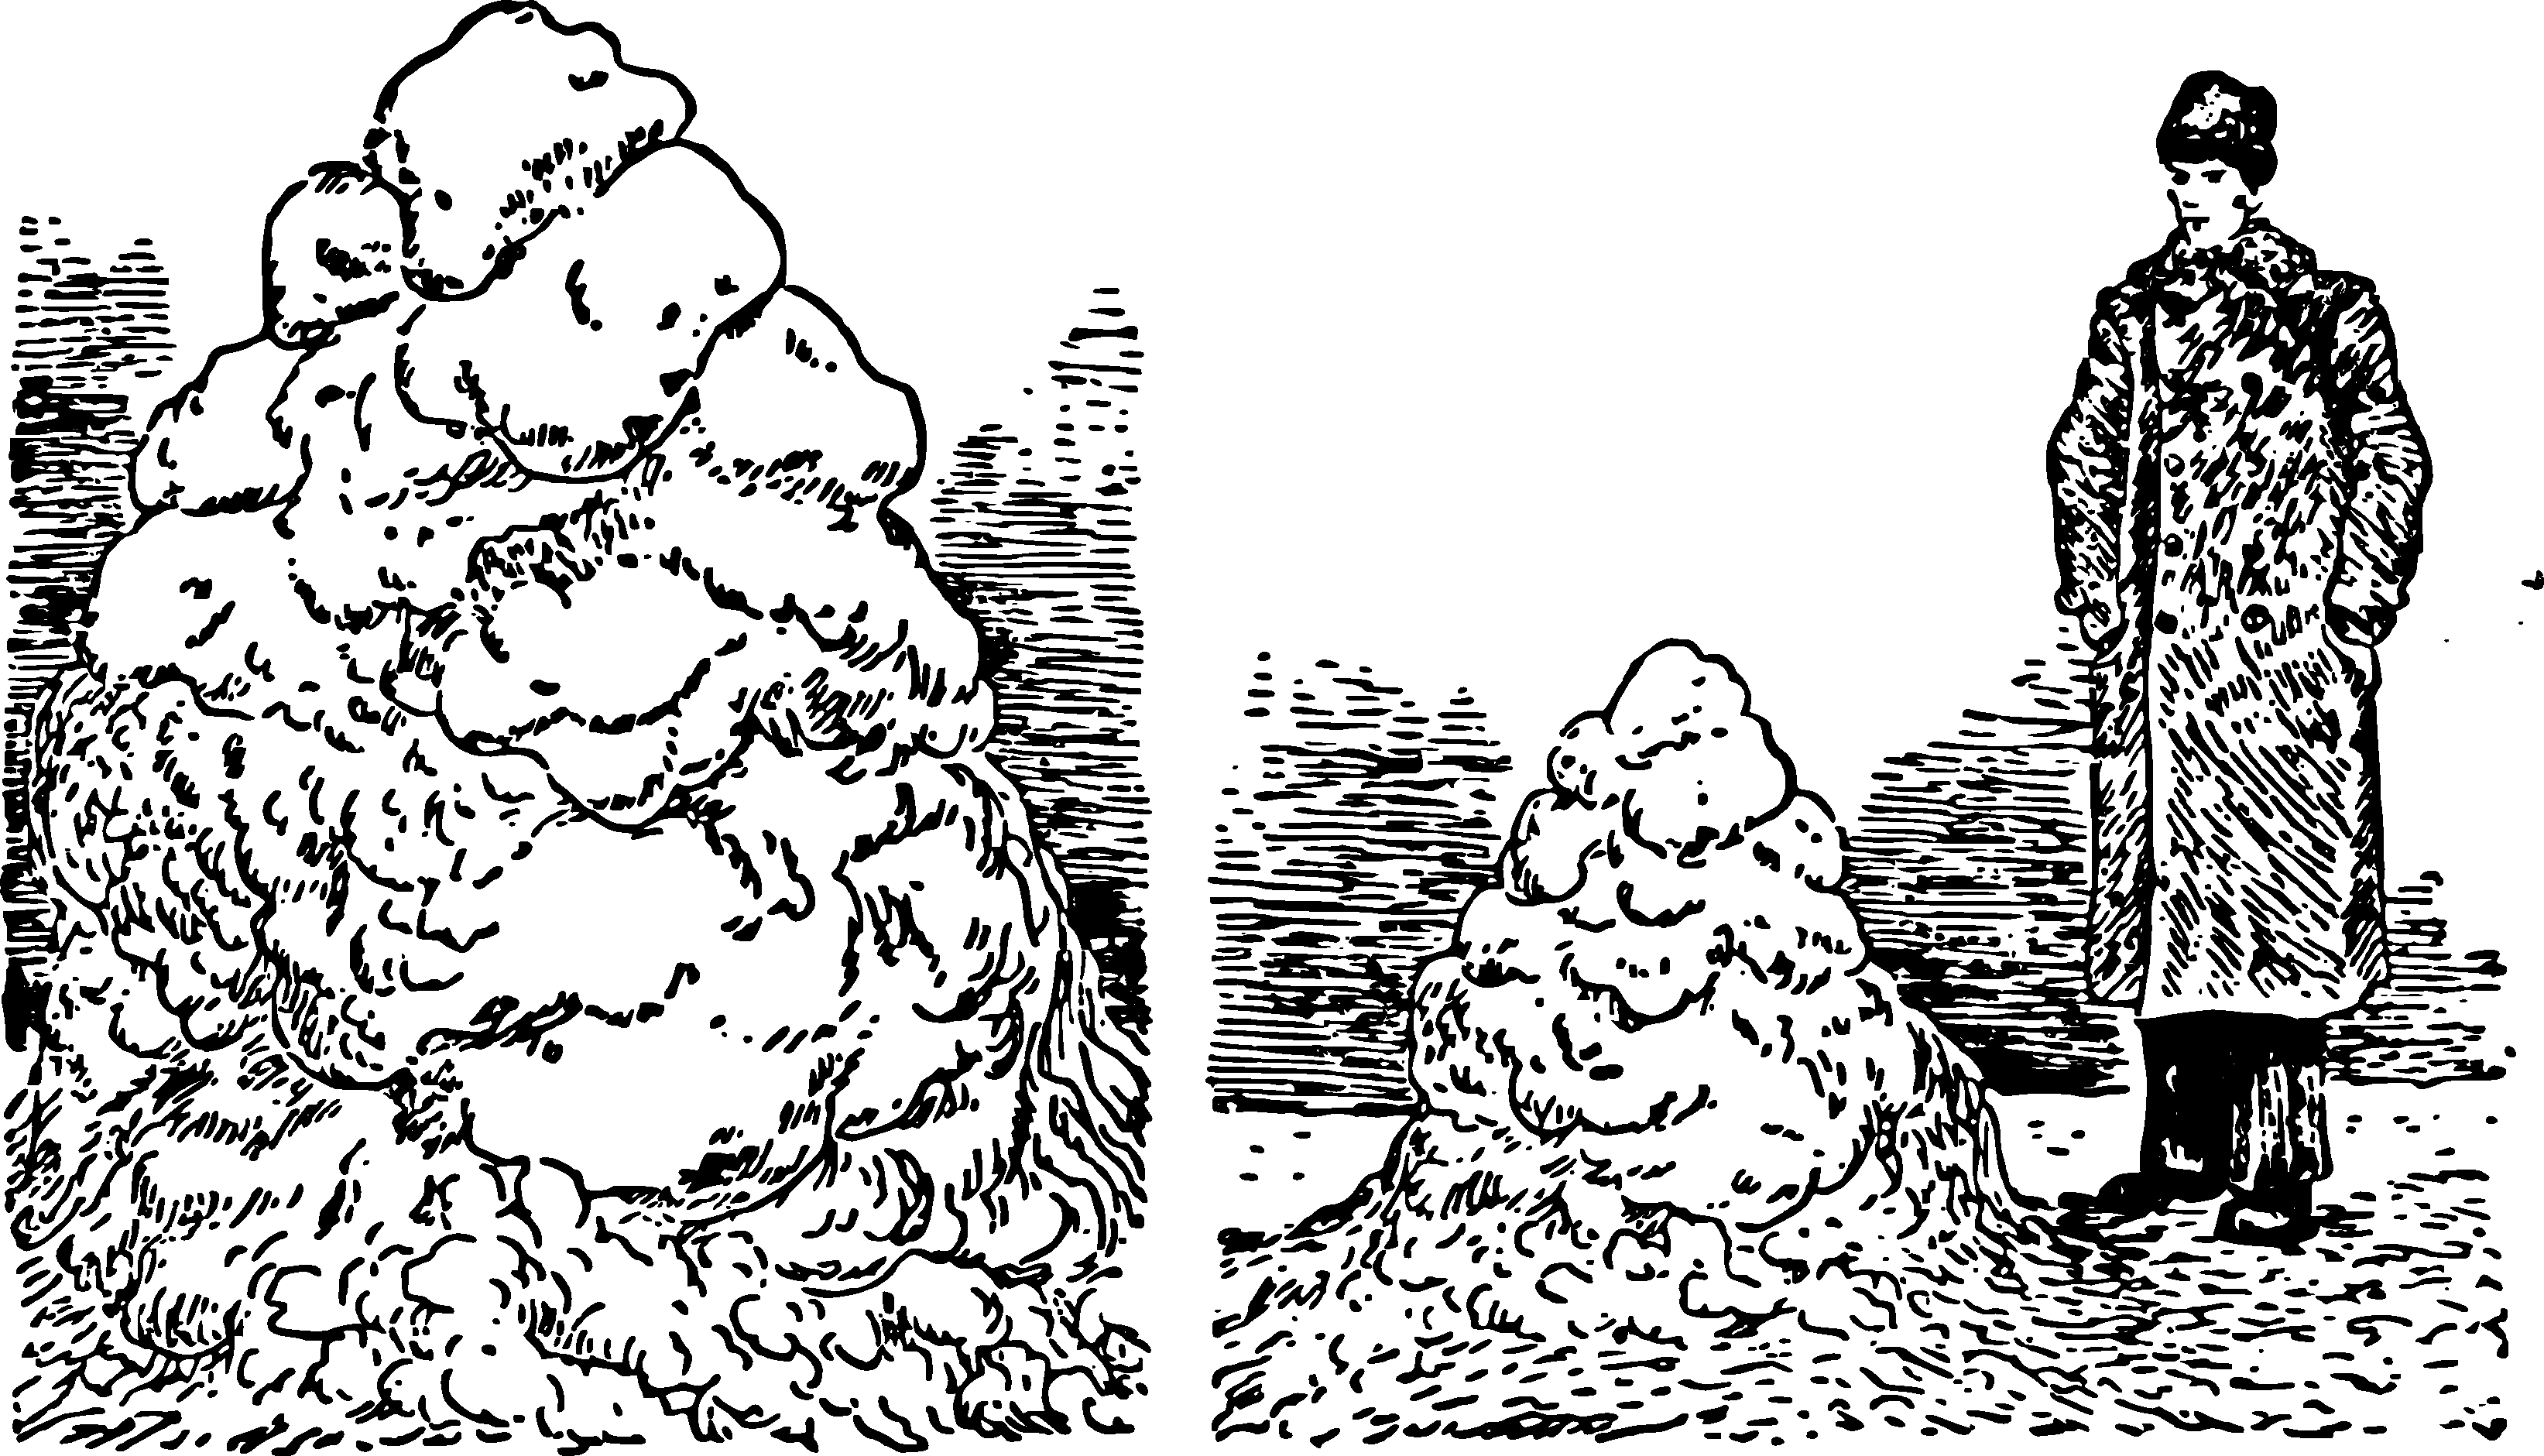
\includegraphics[width=\textwidth]{figures/ch-03/fig-067.pdf}
\sidecaption{Snow mountain in a photograph (left) and in nature (right).\label{fig-067}}
\end{figure}

Another time, the same newspaper reproduced a photo of a wide crevice in the rock near the city; it served, according to the newspaper, as the entrance to an extensive underground cave, where a group of careless tourists who dared to enter the cave for exploration disappeared without a trace. A volunteer search party equipped to search for the lost discovered that the crevice was photographed\dots{} from a barely noticeable crack in the icy wall, a centimetre wide!



\section{Living Protractor}
\label{sec-3.7}

Making a simple protractor device yourself is not very difficult, especially if you use a protractor. But sometimes even a homemade protractor may not be at hand during a countryside walk. In such cases, you can rely on the services of a ``living protractor'' that is always with us. These are our own fingers. To use them for a rough estimate of viewing angles, you just need to make a few preliminary measurements and calculations.

First of all, you need to determine at what angle we see the fingernail of our outstretched index finger. The usual width of a nail is \SI{1}{\centi\meter}, and its distance from the eye in such a position is about \SI{60}{\centi\meter}; therefore, we see it at an angle of about \ang{1} (slightly less because an angle of \ang{1} would be at a distance of \SI{57}{\centi\meter}). For teenagers, the nail is smaller, but the arm is shorter, so the viewing angle for them is approximately the same -- \ang{15}. The reader would do well to perform this measurement and calculation for themselves, relying on book data, to make sure the result is not too far from \ang{15}; if the deviation is significant, you should try another finger.

Knowing this, you have a way to estimate small viewing angles literally with your bare hands. Each distant object, which is just covered by the fingernail of your outstretched index finger, is seen by you at an angle of \ang{1} and, therefore, is 57 times farther away than its width. If the nail covers half of the object, it means its angular size is \ang{2}, and the distance is equal to 28 widths.

The Full Moon covers only half of the nail, i.e., it is seen at an angle of half a degree, meaning it is 114 times its width away from us; here is a valuable astronomical measurement made literally with bare hands!

For larger angles, use the knuckle of your thumb, holding it bent on your outstretched hand. For an adult, the length (note: length, not width) of this joint is about 3.5 cm, and the distance from the eye with an outstretched arm is about 55 cm. It is easy to calculate that the angular size in this position should be about \ang{4}. This provides a means to estimate angles of \ang{4} (and therefore \ang{8}).

Here, you should also add two more angles that can be measured with your fingers -- namely, those under which the intervals between fingers are seen when your middle and index fingers are spread as wide as possible; and between your thumb and index finger, also spread to the maximum. It is easy to calculate that the first angle is approximately \ang{7}-\ang{8}, and the second is \ang{15}-\ang{16}.

There can be many cases to apply your living protractor during walks in open spaces. Suppose a freight car is visible in the distance, which is covered by approximately half of the knuckle of your outstretched thumb, i.e., it is visible at an angle of about \ang{2}. Since the length of a freight car is known (about \SI{6}{\meter}), you can easily find out how far you are from it: $6 \times 28 \approx \SI{170}{\meter}$ or so. A method that does not seem to promise good results, but after a short exercise you will learn to appreciate the services of this ``living ecker''\sidenote{An ``ekker'' is a surveying instrument for drawing lines on the ground at right angles.}, the measurement is, of course, rough, but still more reliable than an ungrounded estimate just by sight.

\begin{figure}[h!]
\centering
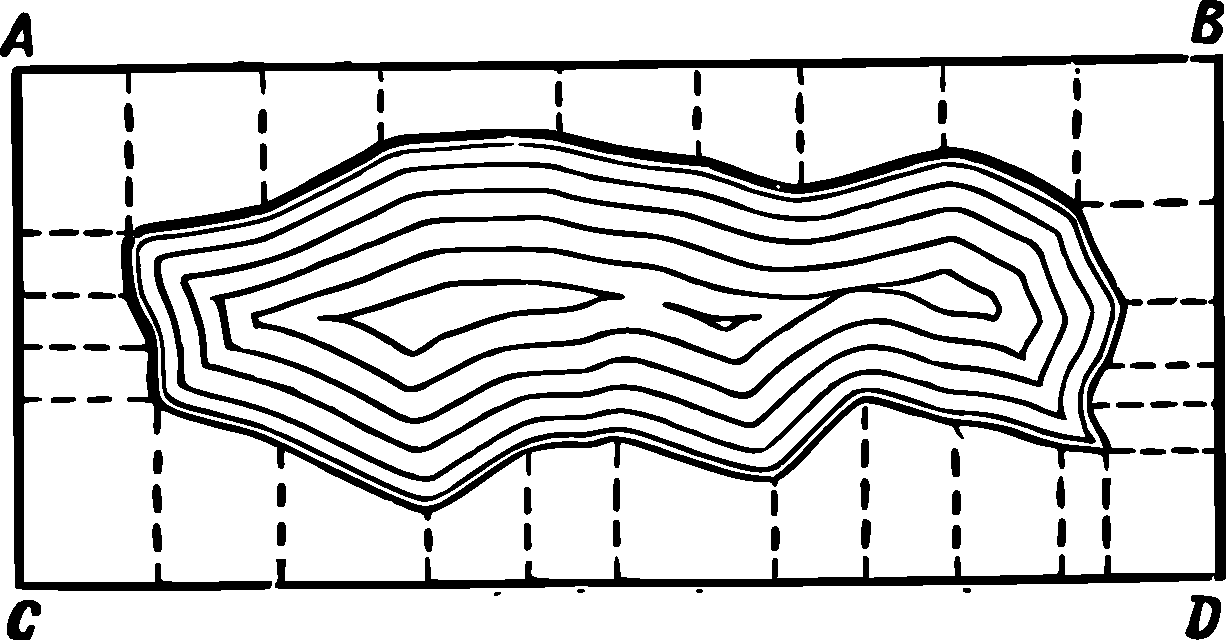
\includegraphics[width=0.8\textwidth]{figures/ch-03/fig-068.pdf}
\sidecaption{Mapping of the lake on the plan.\label{fig-068}}
\end{figure}

Additionally, using your living protractor, you can, in the absence of any tools, measure the angular height of luminaries above the horizon, the mutual separation of stars in degrees, the apparent sizes of a meteor's trail, etc. Finally, knowing how to make right angles on the ground without instruments, you can draw up a plan of a small area using the method whose essence is clear from the illustration, for example, when surveying a lake (\figr{fig-068}), measure rectangle $ABCD$, as well as the lengths of the perpendiculars dropped from prominent points on the shore, and the distances from their bases to the vertices of rectangle $ABCD$. In short, being in Robinson Crusoe's situation, knowing how to use your own hands to measure angles (and your feet to measure distances) could be useful for a variety of needs.

\section{Jacob's Staff}
\label{sec-3.8}

If you wish to have more accurate angle measures than the simple ``living protractor'' described earlier, you can make yourself a simple and convenient device that was once used by our ancestors. This is called ``Jacob's staff'' after its inventor -- a device that was widely used by sailors until the 18th century (\figr{fig-069}), before it was gradually replaced by even more convenient and precise instruments (sextants).

\begin{figure}[h!]
\centering
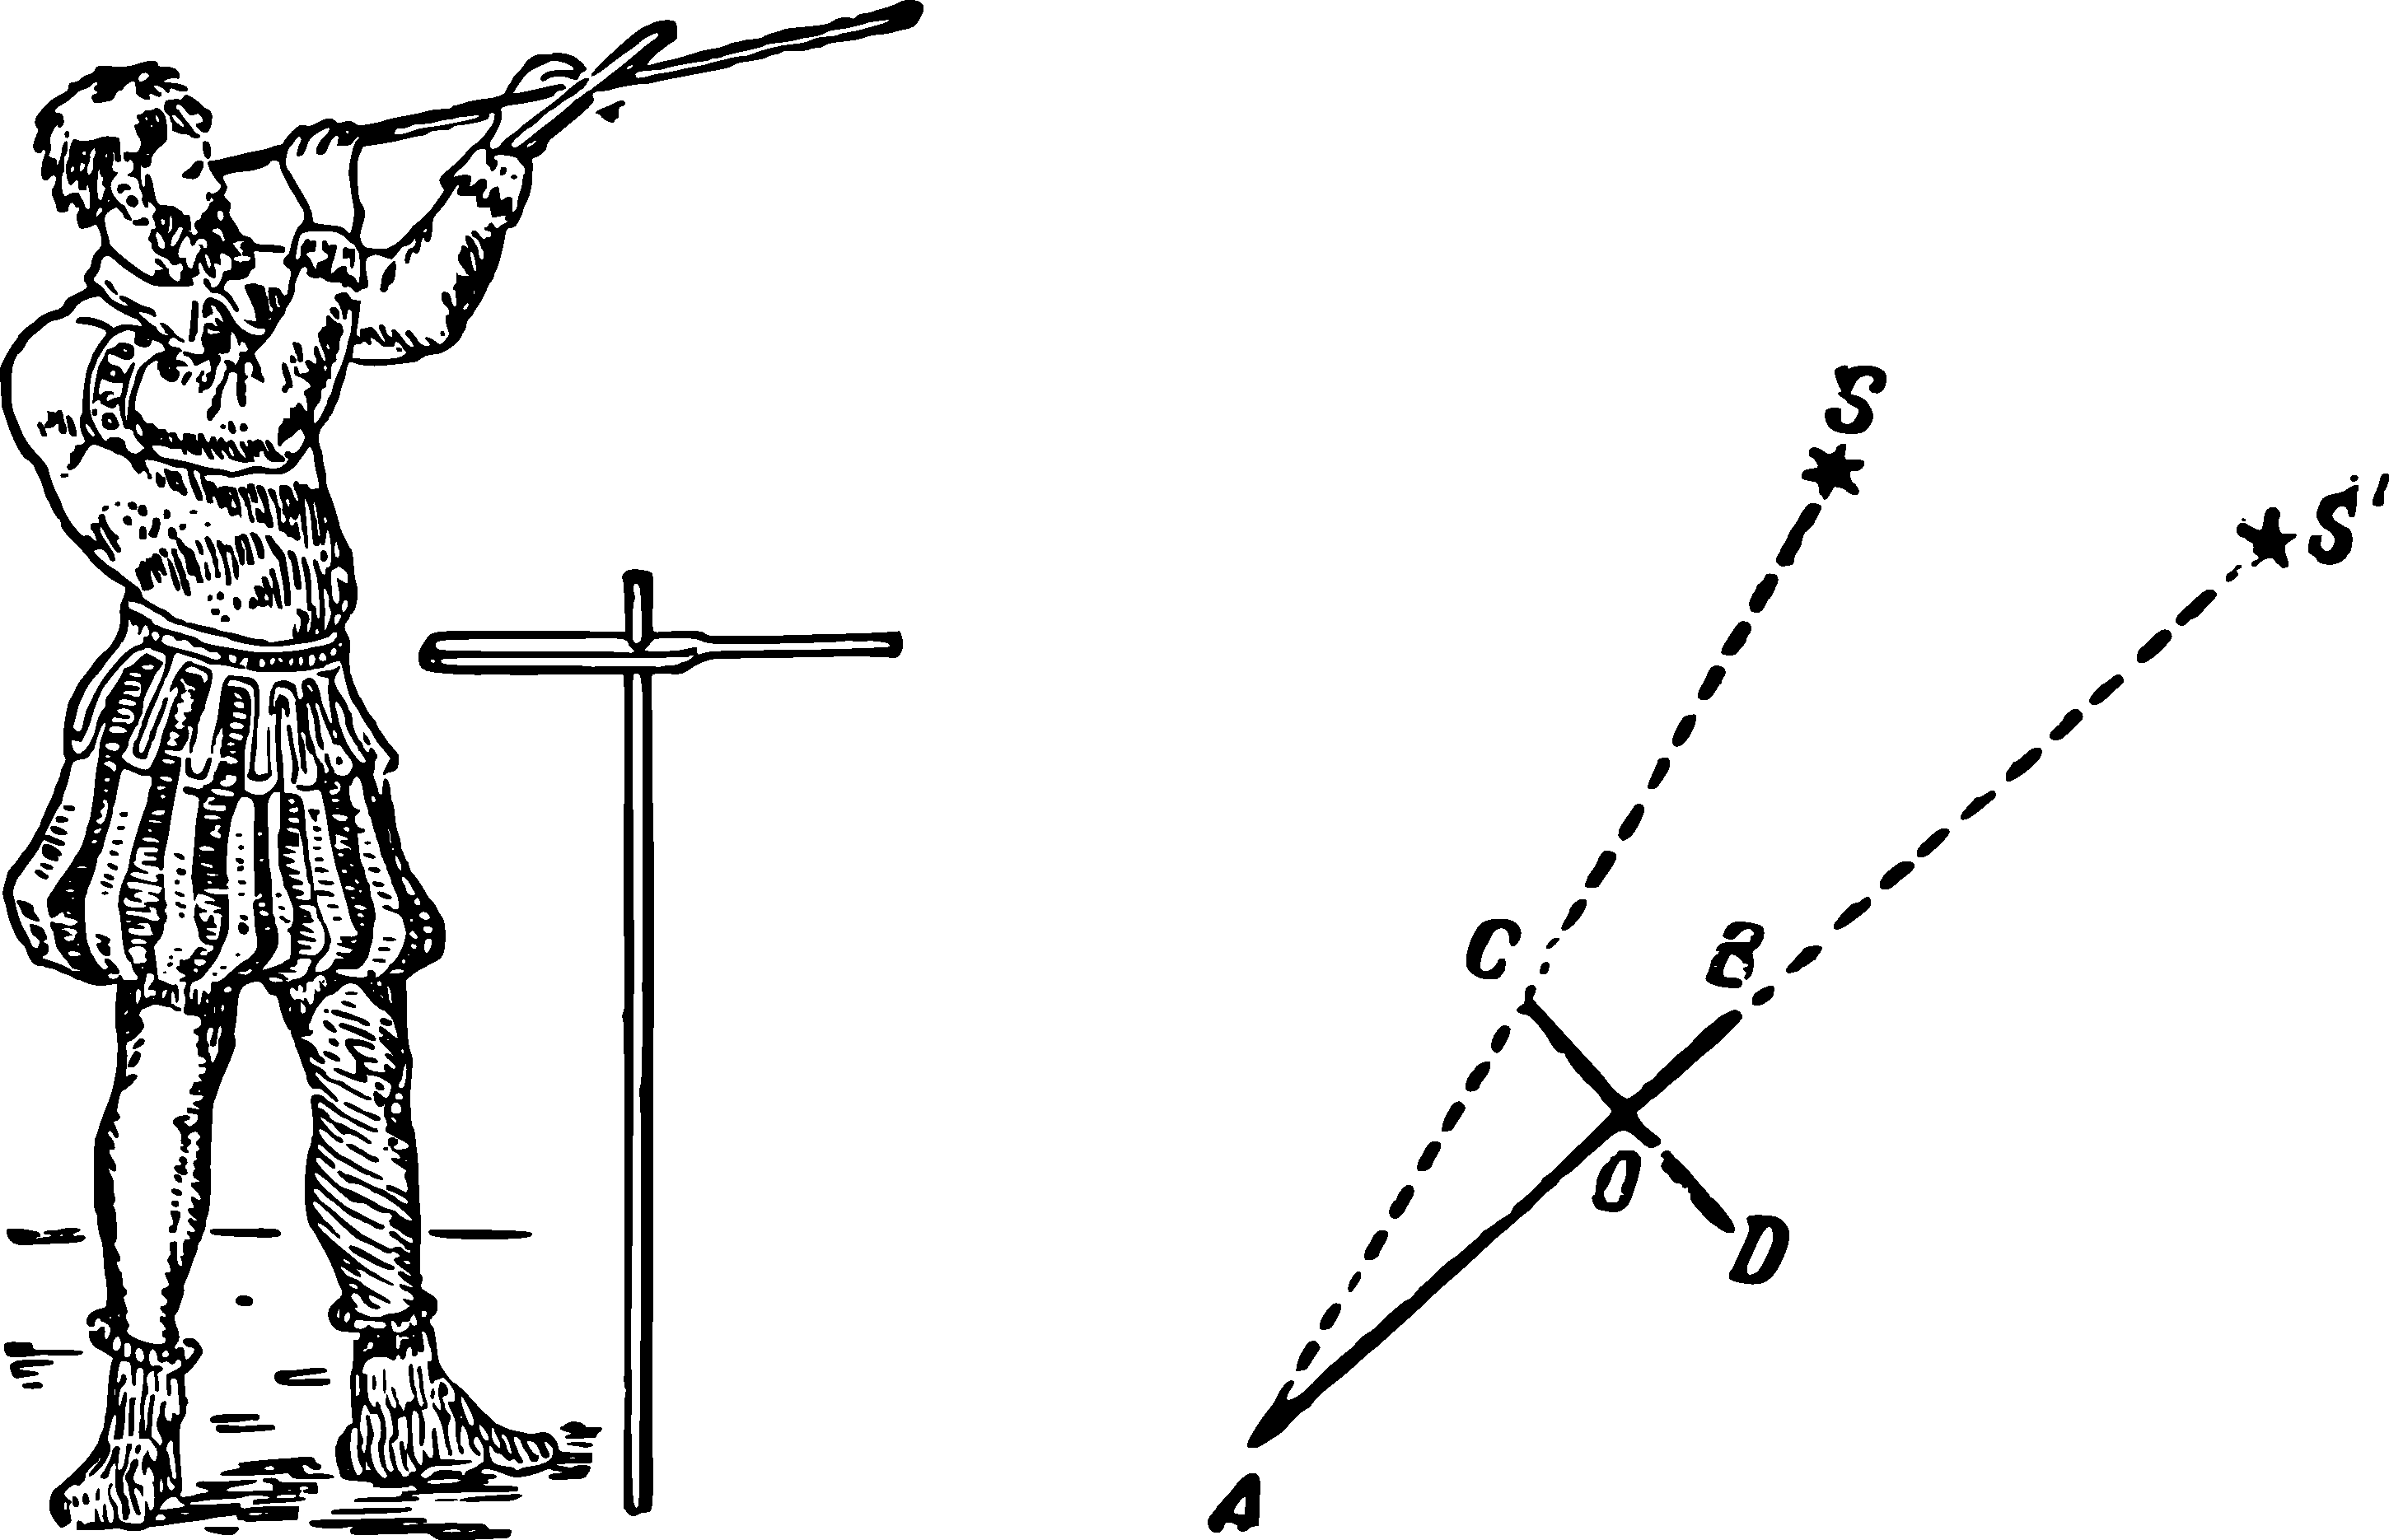
\includegraphics[width=\textwidth]{figures/ch-03/fig-069.pdf}
\sidecaption{Jacob's staff and a diagram of its use.\label{fig-069}}
\end{figure}

It consists of a long ruler $AB$, about 170–100 cm, along which a perpendicular block $CD$ can slide; both parts $CO$ and $OD$ of the sliding block are equal to each other. If you want to determine the angular distance between the stars $S$ and $S'$ using this block (\figr{fig-069}), you attach the end $A$ of the ruler to your eye (where a perforated plate is attached for convenience of observation) and direct the ruler so that the star $S'$ is visible at the end $B$ of the ruler; then you move the crosspiece $CO$ along the ruler until the star $S$ is just visible at the end $C$ (\figr{fig-069}). Now all that remains is to measure the distance $AO$ in order to calculate the value of the angle $SAS'$ using the length of the $CO$. Those familiar with trigonometry will understand that the tangent of the desired angle is equal to the ratio of $CO/AO$. Our ``field trigonometry'', presented in the fifth chapter, is also sufficient for performing this calculation: you calculate the length $AC$ using the Pythagorean theorem, then find angle $C$, whose sine is equal to $CO/AC$.

Finally, you can find the desired angle graphically; by drawing triangle $ACO$ on paper to scale, you measure angle $A$ with a protractor, or if you don't have one, by the method described in our ``field trigonometry'' (see Chapter~\ref{ch-05}).

\begin{figure}[h!]
\centering
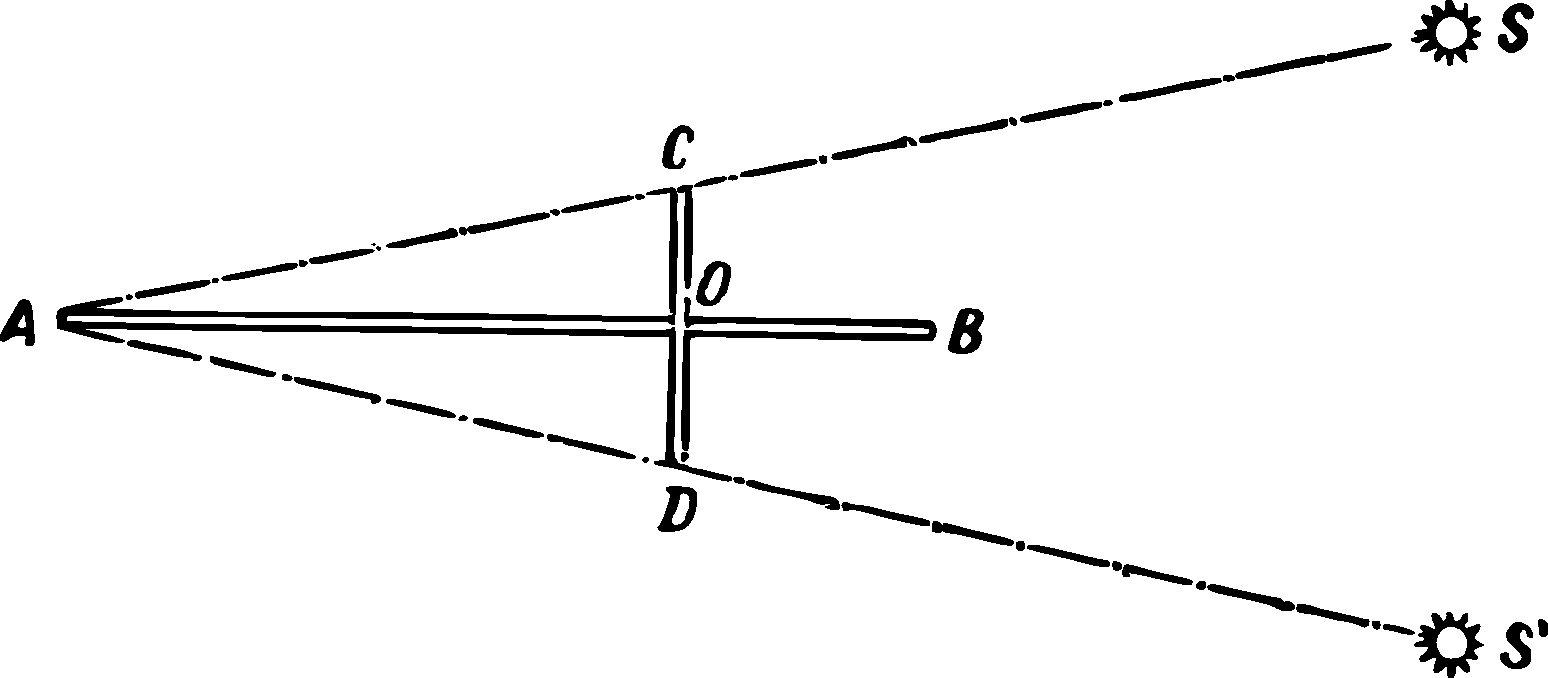
\includegraphics[width=0.9\textwidth]{figures/ch-03/fig-070.pdf}
\sidecaption{Determination of the angular distance between stars using Jacob's staff.\label{fig-070}}
\end{figure}

What is the other half of the crosspiece for? In case the angle to be measured is too large to be measured by the method described above. In that case, instead of directing the ruler $AB$ toward the star $S'$, you aim segment $AD$ toward the point $S'$, moving the crosspiece so that its end $C$ coincides with the star $S$ at the same time (\figr{fig-070}). Finding the angle $SAS'$ by calculation or construction is, of course, not difficult.

To avoid having to make calculations or constructions each time you measure, you can perform them in advance, even when making the device, and mark the results on the ruler $AB$; then, when aiming the device at the stars, you only need to read the reading recorded at point $O$ — this is the value of the measured angle.


\section{Rake Angle Gauge}
\label{sec-3.9}

It's even easier to make another device for measuring angular magnitude -- the so-called `rake angle gauge,' which indeed resembles a rake in appearance (\figr{fig-071}). Its main part is a board of any shape, with a drilled plate attached at one end; the observer aligns their eye with its hole. At the opposite end of the board, a row of thin pins\sidenote{Instead of pins, you can use a frame with strands stretched on it.} (commonly used for insect collections) is inserted, the gaps between which make up the 57th part of their distance from the hole of the drilled plate. It is already known that each interval is observed at an angle of one degree. One can also place the pins using another method, yielding a more precise result: two parallel lines are drawn on the wall, one meter apart, and stepping back from the wall perpendicular to them by 57 m, these lines are viewed through the hole in the drilled plate; the pins are inserted into the board so that each pair of adjacent pins covers the lines drawn on the wall.

\begin{figure}[h!]
\centering
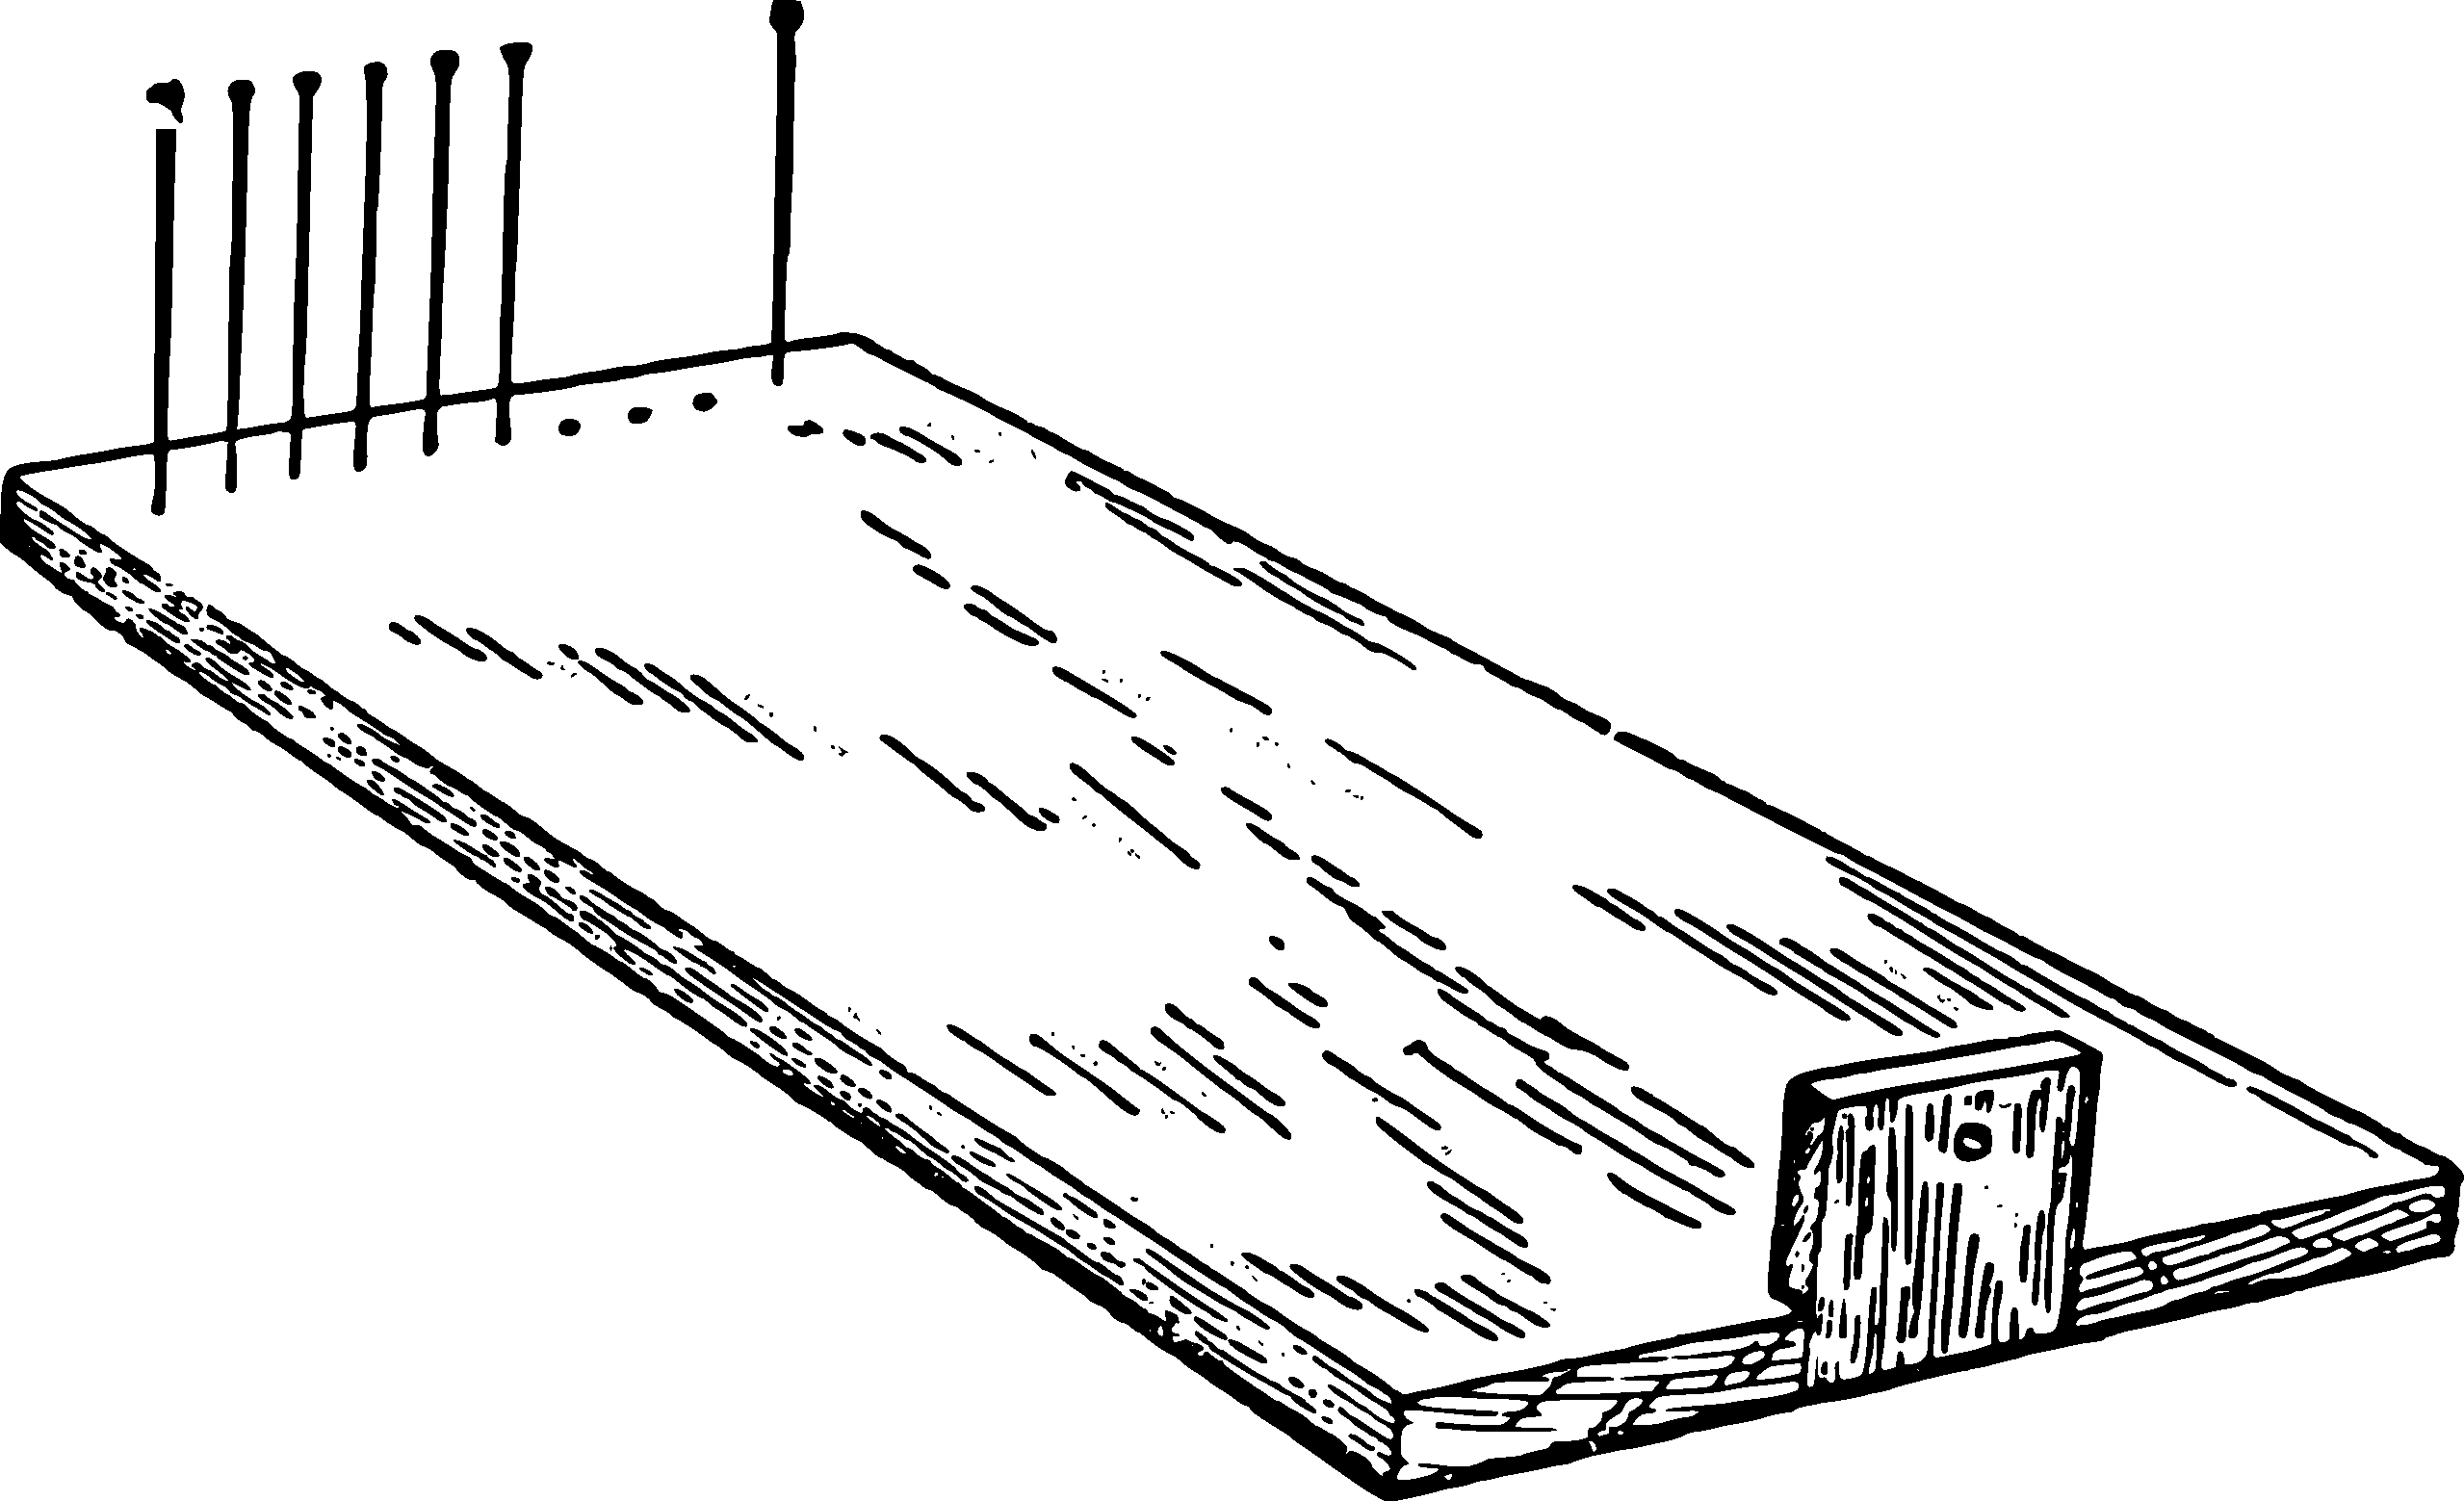
\includegraphics[width=0.9\textwidth]{figures/ch-03/fig-071.pdf}
\sidecaption{A rake protractor.\label{fig-071}}
\end{figure}

Once the pins are placed, some of them can be removed to obtain angles of \ang{2}, \ang{3}, \ang{5}. The method of using this angle gauge is, of course, understandable to the reader even without explanations. By using this angle gauge, angles of view can be measured with quite high accuracy, no less than \ang{0.25}.

\section{Artilleryman's Angle}
\label{sec-3.10}

An artilleryman does not shoot `blindly'. Knowing the position of the target, he determines its angular magnitude and calculates the distance to the target; in another case, he determines at what angle he needs to turn the gun to shift fire from one target to another. He solves such tasks quickly and mentally. How? Look at \figr{fig-072}, $AB$ is the arc of circle from $OA = D$; $ab$ - the arc of circle with radius $Oa = r$. From the similarity of the two sectors $AOB$ and $aOB$ it follows
\begin{align*}%
\frac{AB}{D} & = \frac{ab}{r}, \qor \\ 
AB & = \frac{ab}{r}\, D.
\end{align*}
The ratio $ab/r$ characterises the angle of view $AOB$; knowing this ratio, it is easy to calculate $AB$ from a known $D$ or $D$ from a known $AB$.

\begin{figure}[h!]
\centering
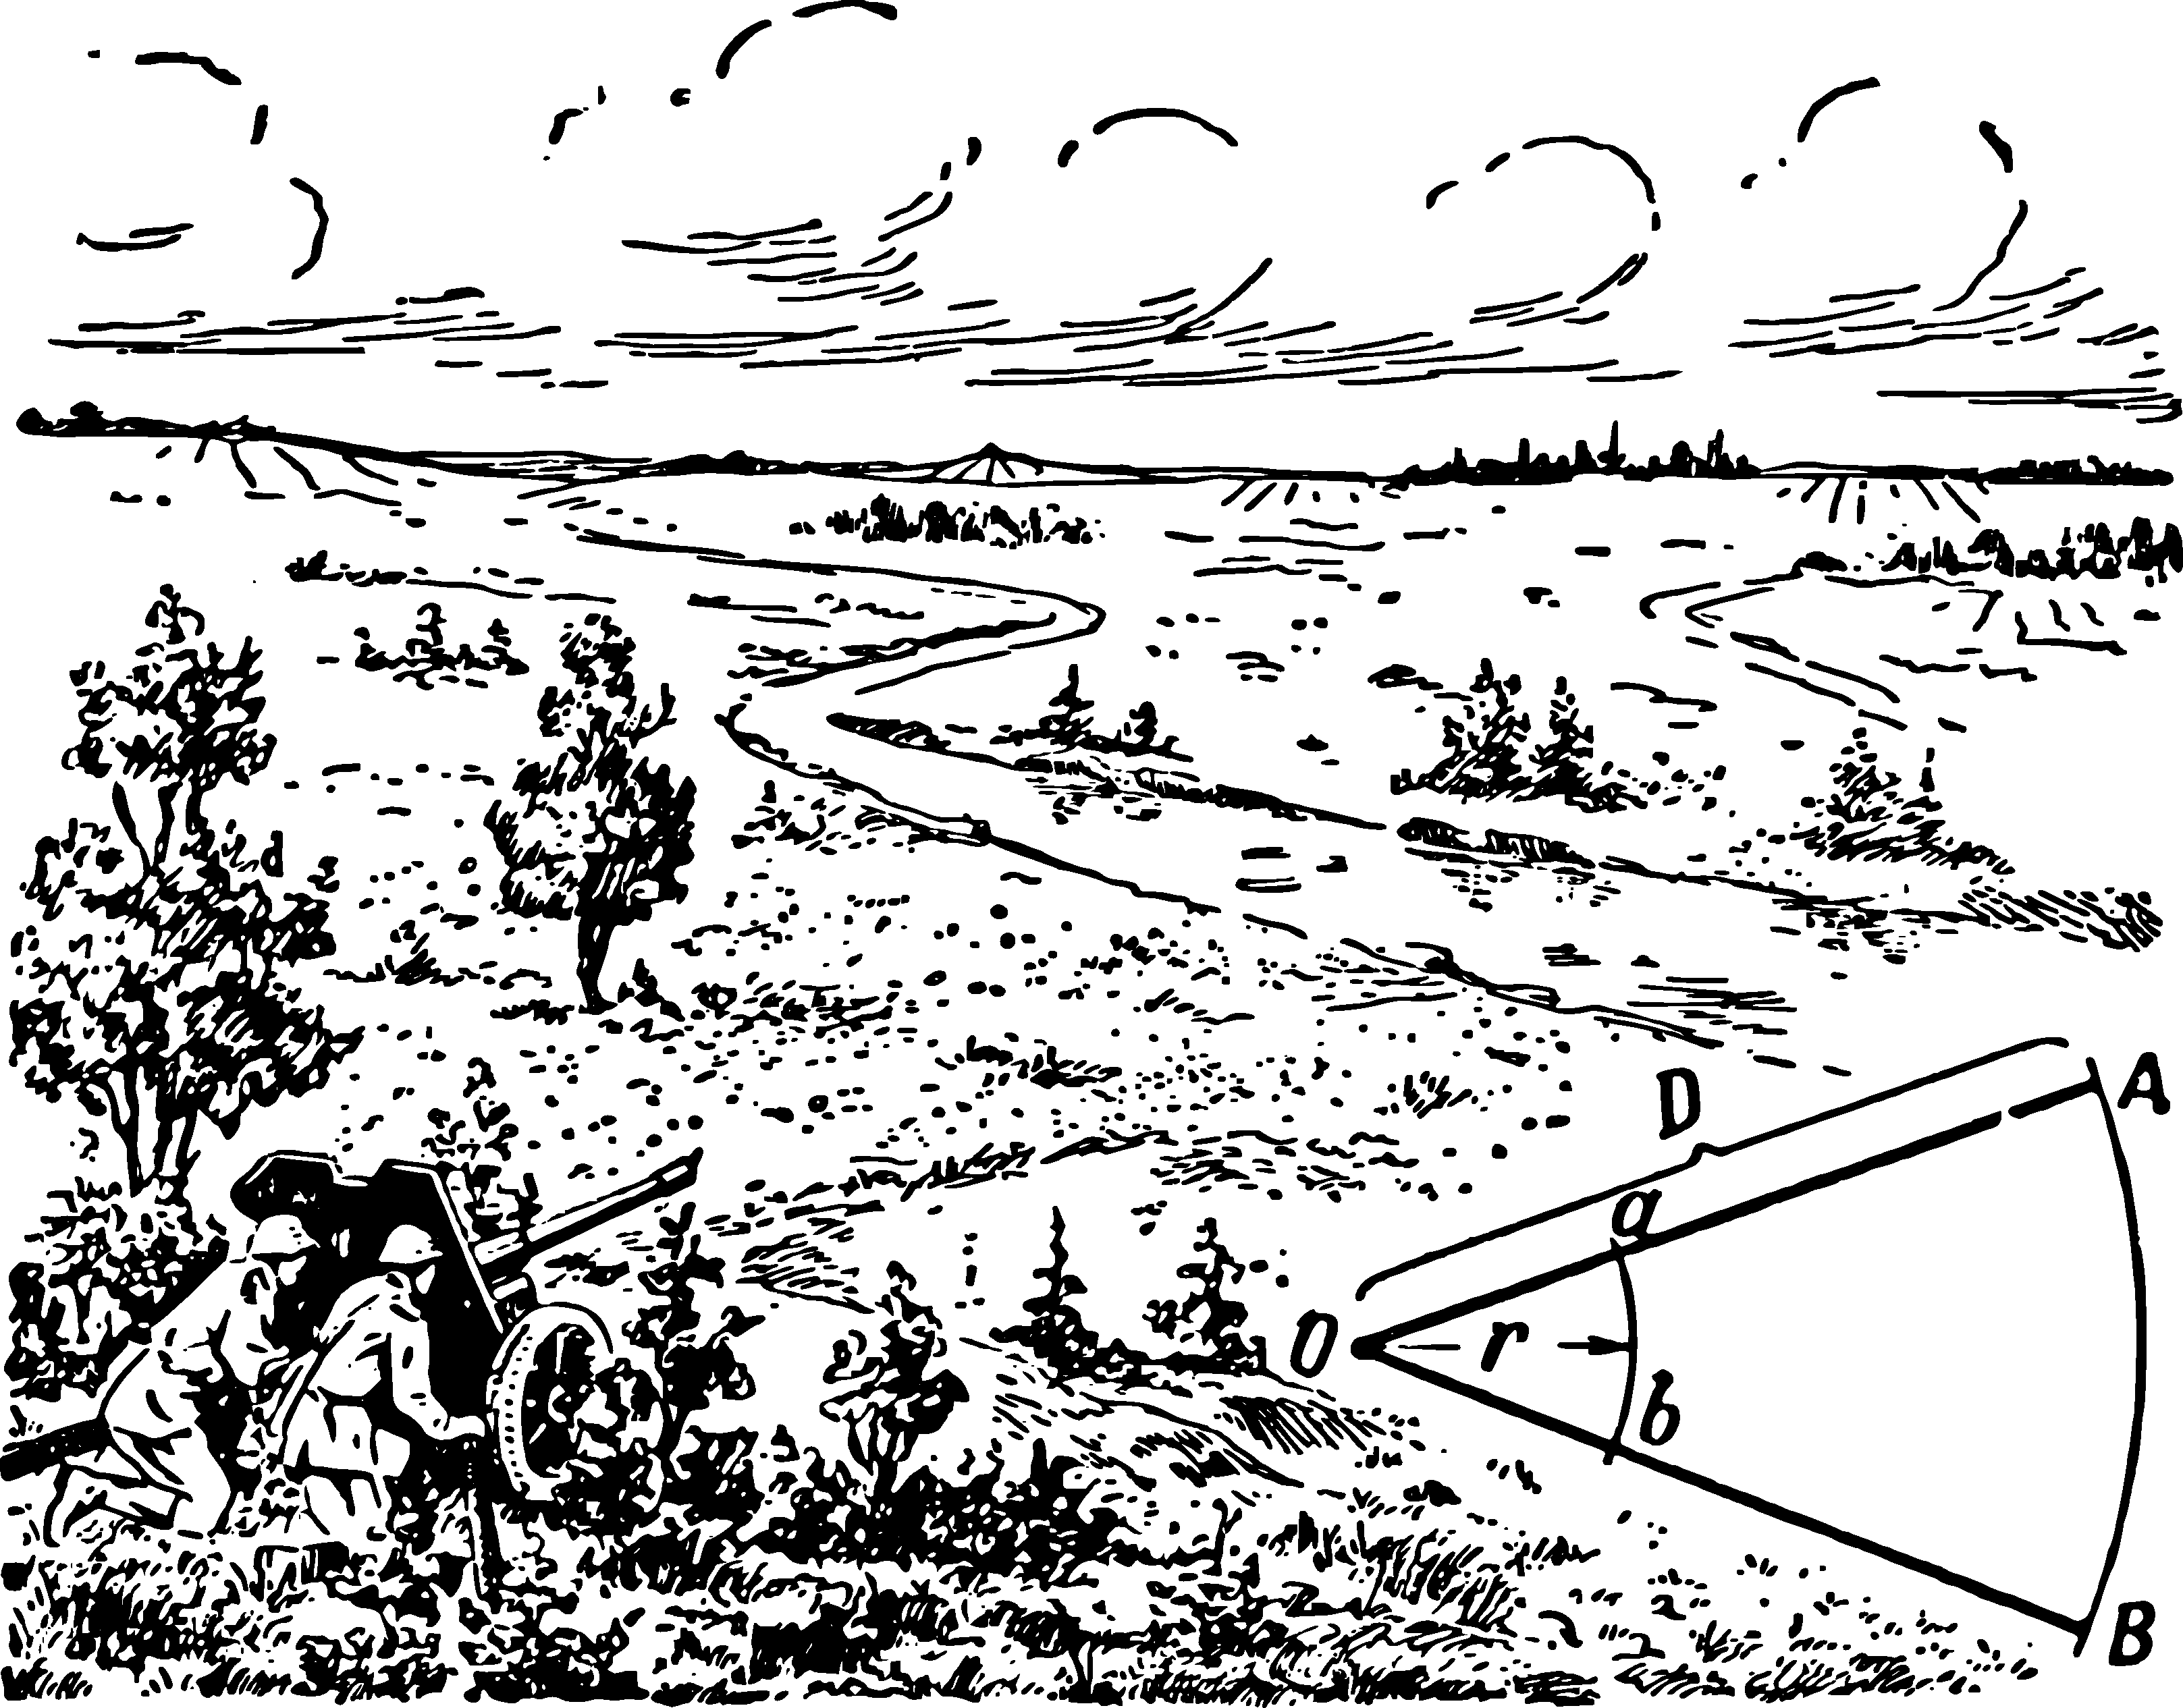
\includegraphics[width=0.9\textwidth]{figures/ch-03/fig-072.pdf}
\sidecaption{A rake protractor.\label{fig-072}}
\end{figure}


Artillerymen facilitate their calculations by dividing the circle not into 360 parts, as usual, but into 6000 equal arcs. Then the length of each division is approximately 1/1000 times the radius of the circle. Indeed, let, for example, the arc $ab$ of the angle circle $O$ (\figr{fig-072}) represent one unit of division; then the length of the entire circumference $2 \pi r \approx 6r$, and the length of the arc $ab = 6r/6000 = 1/1000 \, r$.

In artillery, it is called a `thousandth'. So,
\begin{equation*}%
AB = \frac{0.001\,r}{r} \, D = 0.001 \, D,
\end{equation*}
i.e., to find out what distance $AB$ on the ground corresponds to one division of the angle-measurer (angle in one `thousandth'), it is sufficient in the distance $D$ to move the decimal point three digits to the right.

When transmitting commands or observation results by field telephone or radio, the number of `thousandths' is pronounced like a telephone number, for example: an angle of 105 `thousandths' is pronounced: `one zero five', and written as: 
\begin{equation*}%
1-05;
\end{equation*}
an angle of 8 `thousandths' is pronounced: 'zero zero eight', and written as:
\begin{equation*}%
1-08.
\end{equation*}
Now you can easily solve such an artillery problem.


\ques The tank (in terms of height) is visible from the anti-tank gun at an angle of $0-05$. Determine the distance to the tank, assuming its height is 2 meters.

\ans 
\begin{align*}%
\text{5 divisions of the angle-measurer} & = \SI{2}{\meter},\\
\text{so 1 division of the angle-measurer} & = \frac{\SI{2}{\meter}}{5} = \SI{0.4}{\meter}. 
\end{align*}
Since one division of the angle-measurer corresponds to one thousandth of the distance, the entire distance is therefore a thousand times greater, i.e.,
\begin{equation*}%
D = 0.4 \times 1000 = \SI{400}{\meter}.
\end{equation*} 
If the commander or scout does not have an angle-measuring device at hand, they use their palm, fingers, or any other improvised means, as described in our book (\hyperref[sec-3.7]{Living Protractor}). However, their ``value'' must be given to the artilleryman not in degrees, but in ``thousandths''. Here is the approximate ``value'' in ``thousandths'' of some items:


\begin{small}
\begin{tabular}{p{5cm}p{1.75cm}}
\toprule
Object & Angle in `thousandths'\\
\midrule 
Palm of the hand (average) & $ 1-20$\\
Middle, index, or ring finger& $ 0-30$\\
Round pencil (thickness)& $0-12$\\
Three-kopeck or twenty-kopeck coin (diameter)&  $0-40$\\
Matchstick (length) & $0-75$\\
Matchstick (thickness) & $0-03$\\
\bottomrule
\end{tabular}
\end{small}


\section{Your visual acuity}
\label{sec-3.11}

Once you grasp the concept of angular magnitude of an object, you will understand how visual acuity is measured, and even perform such measurements yourself.

Draw on a piece of paper 20 equally spaced black lines each as long as a matchstick (\SI{5}{\centi\meter}) and one millimetre thick, so that they fill a square (see \figr{fig-073}). Attach this drawing to a well-lit wall and step away from it until you notice that the lines are no longer individually distinguishable, but merge into a continuous grey background. Measure this distance and calculate -- as you already know how to do -- the angle of vision under which you cease to distinguish the stripes at \SI{1}{\milli\meter} thickness. If this angle is \ang{;1} (one minute), then your vision acuity is normal; if it is three minutes -- your acuity is ``below normal'' and so on.

\begin{marginfigure}%[h!]
\centering
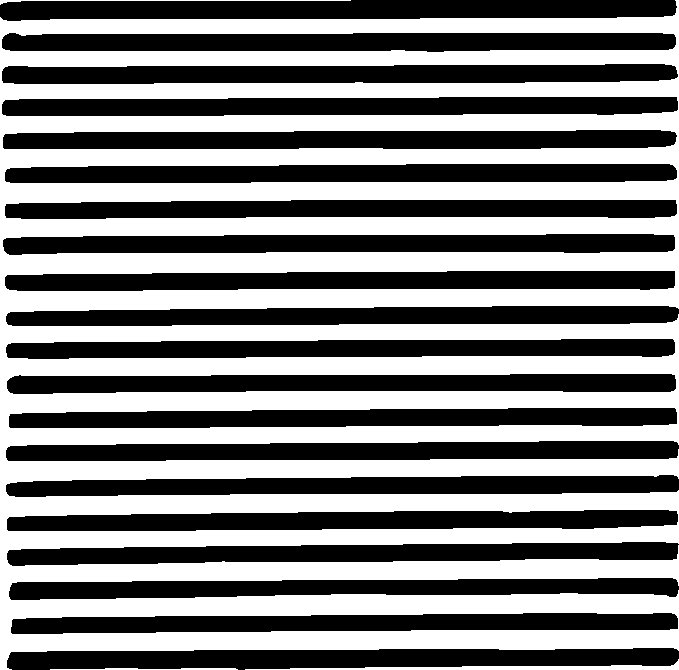
\includegraphics[width=\textwidth]{figures/ch-03/fig-073.pdf}
\sidecaption{To measure visual acuity.\label{fig-073}}
\end{marginfigure}



\ques Lines in \figr{fig-073} merge for your eye at a distance of \SI{2}{\meter}. Is vision acuity normal? 

\ans We know that from a distance of \SI{57}{\milli\meter}, a stripe with a width of \SI{1}{\milli\meter} is visible at an angle of \ang{1}, i.e., \ang{;60}. Therefore, from a distance of \SI{2000}{\milli\meter}, it is visible at an angle $x$ which is determined from the proportion 
\begin{equation*}%
\frac{x}{60} = \frac{57}{2000}, \quad x = \ang{;1.7}
\end{equation*}
Vision acuity is below normal and amounts to
\begin{equation*}%
\frac{1}{1.7} \approx 0.6.
\end{equation*}


\section{The Limiting Minute}
\label{sec-3.12}

We've just mentioned that stripes viewed at an angle of less than one minute cease to be individually distinguishable by a normal eye. This holds true for any object: regardless of the contours of the observed object, they cease to be distinguishable by a normal eye if they are visible at an angle less than \ang{;1}. Each object becomes a barely distinguishable point, ``too small for sight'' (Shakespeare), a speck without size or shape. This is a property of the normal human eye: one angular minute is the average limit of its acuity. What causes this is a special question related to the physics and physiology of vision. We only discuss the geometric aspect of the phenomenon here.

The same applies equally to large but distant objects and to close but too small ones. We cannot distinguish with the naked eye the shapes of dust particles floating in the air: illuminated by sunlight, they appear to us as identical tiny dots, although in reality, they have a variety of shapes. We cannot discern small details of an insect's body for the same reason, because we see them at an angle less than \ang{;1}. For the same reason, without a telescope, we do not see the details on the surface of the Moon, planets, and other celestial bodies.

The world would seem completely different to us if the boundary of natural vision were pushed further. A person whose limit of visual acuity is not \ang{;1}, but, for example, \ang{;0.5}, would see the surrounding world deeper and farther than we do. Chekhov vividly described this advantage of sharp eyesight in his story \emph{The Steppe}.

``His (Vasya's) vision was remarkably sharp. He saw so well that the brown barren steppe was always full of life and content for him. He only had to look into the distance to see a fox, a hare, a bustard, or some other animal, keeping itself away from people. It was not difficult to see a fleeing hare or a flying bustard -- anyone passing through the steppe could see them -- but not everyone could see wild animals in their domestic life, when they are not running, hiding, or looking around anxiously. And Vasya saw playing foxes, hares washing their paws, bustards spreading their wings, and snipes drumming. Thanks to such keen vision, besides the world that everyone saw, Vasya had another world, his own, inaccessible to anyone else, and probably very good, because when he looked and admired, it was difficult to envy him."

It's strange to think that such a remarkable change is sufficient by simply lowering the limit of discernibility from \ang{;1} to \ang{;0.5} or so \dots{}

The magical effect of microscopes and telescopes is also due to the same reason. The purpose of these instruments is to alter the course of rays from the observed object so that they enter the eye with a more divergent beam; thanks to this, the object appears at a larger angle of vision. When it is said that a microscope or telescope magnifies by 100 times, it means that with their help, we see objects at an angle 100 times larger than with the naked eye. And then the details hidden from the naked eye beyond the limit of acuity become accessible to our sight. 

We see the full moon at an angle of \ang{;30}'; and since the diameter of the Moon is \SI{3500}{\kilo\meter}, then each area of the Moon with a diameter of $3500/30$, i.e., about \SI{120}{\kilo\meter}, merges into a barely distinguishable point for the naked eye. In a telescope, which magnifies by 100 times, much smaller areas with a diameter of $120/100 = \SI{1.2}{\kilo\meter}$ will already be indistinguishable, and in a telescope with a 1000-fold magnification -- an area of \SI{120}{\meter} wide. Hence, among other things, if there were such constructions on the Moon as our large plants or ocean liners, we could see them through modern telescopes.\sidenote[][-2cm]{Under the condition of full transparency and uniformity of our atmosphere. In reality, the air is not homogeneous and not entirely transparent; therefore, at high magnifications, the visible picture becomes hazy and distorted. This imposes a limit on the use of very strong magnifications and prompts astronomers to build observatories in the clear air of high mountain peaks.}

The rule of the limiting minute has a significant effect on our ordinary everyday observations as well. Due to this feature of our vision, every object, distant by 3400 (i.e., $57 \times 60$) of its diameter, ceases to be distinguished by us in its outlines and merges into a point. Therefore, if someone claims that they recognised a person's face with the naked eye from a distance of a quarter of a kilometre, do not believe them -- unless they have phenomenal vision. After all, the distance between a person's eyes is only \SI{8}{\centi\meter}; this means that both eyes merge into a point already at a distance of $3 \times \SI{3400}{\centi\meter}$, i.e., \SI{100}{\meter}. Artillerymen use this for visual estimation of distance. According to their rules, if a person's eyes appear as two separate points from a distance, then the distance to them does not exceed 100 steps (i.e., 60-70 m). We obtained a greater distance -- 100 m: this shows that the military sign indicates somewhat reduced (to 30\%) visual acuity.

\ques Can a person with normal vision distinguish a rider at a distance of 10 km, using binoculars magnifying three times?

\ans The height of the rider is 2.2 m. His figure turns into a point for the naked eye at a distance of $2.2 \times 8400 = \SI{7}{\kilo\meter}$; in binoculars magnifying three times -- at a distance of 21 km. Therefore, it is possible to distinguish him at distance of 10 km with such binoculars (if the air is sufficiently transparent).
\clearpage

\section{The Moon and Stars at the Horizon}
\label{sec-3.13}

Even the most inattentive observer knows that the full moon, hanging low at the horizon, appears noticeably larger than when it is high in the sky. The difference is so significant that it's hard not to notice. The same holds true for the Sun; it's well-known how large the solar disk appears at sunset or sunrise compared to its size high in the sky, for example, when it shines through the clouds (directly looking at the unobscured sun is harmful to the eyes).

For stars, this peculiarity manifests in the way the distances between them increase as they approach the horizon. Anyone who has seen the beautiful constellation Orion in winter (or Cygnus in summer) high in the sky and low near the horizon cannot help but be struck by the enormous difference in the constellation's size in both positions.


All this is made more mysterious by the fact that when we look at celestial bodies at sunrise or sunset, they are not only not closer but, on the contrary, farther away (by the size of the Earth's radius), as easily understood from \figr{fig-074}: at the zenith, we view the celestial body from point $A$, and at the horizon -- from points $B$ or $C$. So why do the Moon, the Sun, and constellations appear larger at the horizon?


\begin{figure}[h!]
\centering
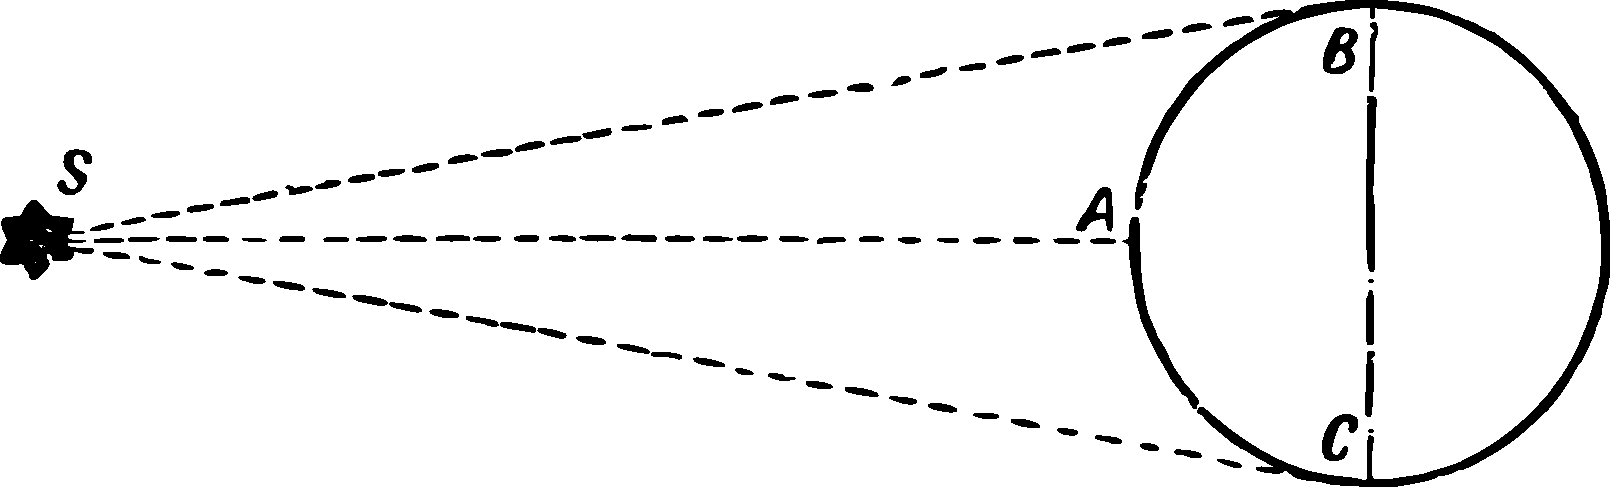
\includegraphics[width=\textwidth]{figures/ch-03/fig-074.pdf}
\sidecaption{Why is the Sun, being on the horizon, farther from the observer than being in the middle of the sky.\label{fig-074}}
\end{figure}


One might answer, ``Because it's not true.'' It's a visual deception. With the help of a protractor or another angle-measuring instrument, it's easy to verify that the lunar disk is visible in both cases at the same angular size (half a degree)\sidenote{Measurements made with more precise instruments show that the visible diameter of the Moon is even smaller when the Moon is near the horizon, due to the fact that refraction slightly flattens the disk.}. Using the same device or ``Jacob's staff,'' one can ascertain that the angular distances between stars do not change, regardless of whether the constellation is at the zenith or the horizon. Therefore, the enlargement is an optical illusion to which all people are subject without exception.

What explains such a strong and universal visual deception? Science has not yet provided a definitive answer to this question, as far as we know, although it has been striving to resolve it for 2000 years, since the time of Ptolemy. The illusion is related to the fact that we perceive the entire celestial sphere not as a hemisphere in the geometric sense but as a spherical segment, the height of which is 2–3 times smaller than the radius of the base. This is because with our head and eyes in their usual position, distances in the horizontal direction and close to it are perceived by us as more significant compared to vertical ones: in the horizontal direction, we view an object ``directly'', while in any other direction — with eyes raised upwards or lowered downwards. If one observes the Moon while lying on one's back, it will appear larger when it is at the zenith than when it stands low above the horizon.\sidenote{In previous editions of \emph{Entertaining Geometry}, Ya. I. Perelman explained the apparent enlargement of the Moon at the horizon by the fact that at the horizon, we see it next to distant objects, while in the empty celestial vault, we see it alone. However, the same illusion is observed on the unfilled horizon of the sea, so the previously proposed explanation of the described effect must be considered unsatisfactory.}

\begin{figure}[h!]
\centering
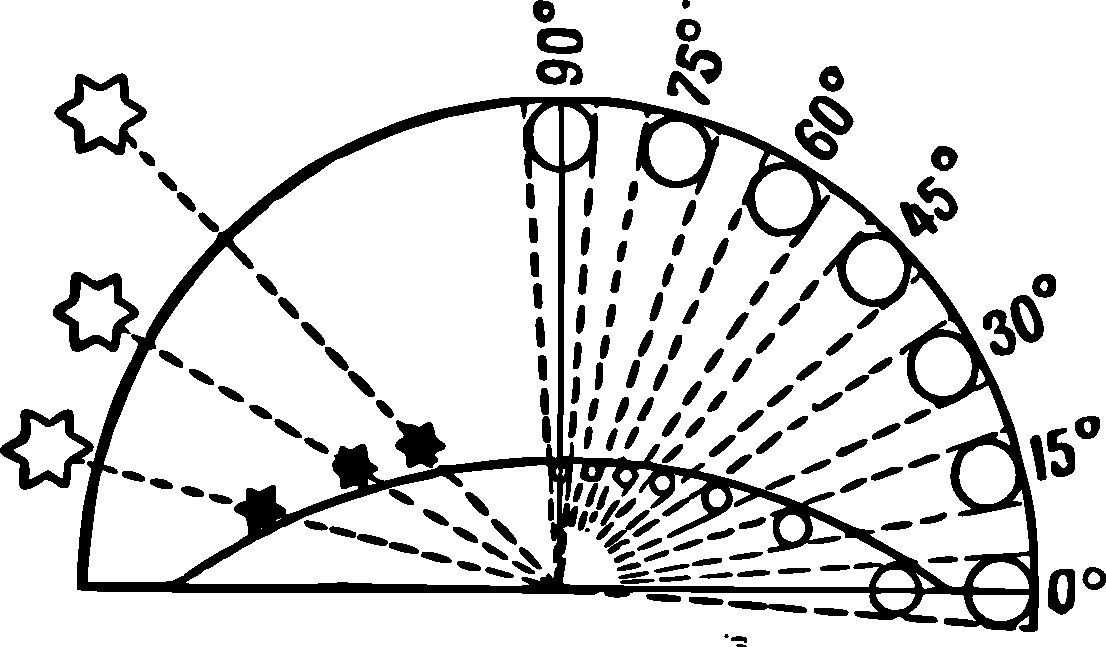
\includegraphics[width=0.8\textwidth]{figures/ch-03/fig-075.pdf}
\sidecaption{The influence of the flatness of the firmament on the apparent size of the celestial objects.\label{fig-075}}
\end{figure}


Psychologists and physiologists are faced with the task of explaining why the visible size of an object depends on the orientation of our eyes. As for the influence of the apparent flattening of the celestial sphere on the size of celestial bodies in its different parts, it becomes quite understandable from the scheme depicted in \figr{fig-075}. The lunar disk is always visible at an angle of half a degree in the celestial vault, whether the Moon is at the horizon (at an altitude of \ang{0}) or at the zenith (at an altitude of \ang{90}). However, our eye refers this disk not always to the same distance: the Moon at the zenith is perceived by us as being closer than at the horizon, and therefore its size seems different -- within the same angle, a smaller circle is placed closer to the vertex than farther from it. On the left side of the same figure, it is shown how, due to this reason, the distances between stars seem to stretch as they approach the horizon: when the angular distances between them are the same, they seem different.

There is another instructive aspect here. Admiring the huge lunar disk near the horizon, have you noticed any new features on it that you couldn't discern on the disk of the moon standing high? No. But before you is an enlarged disk, so why aren't new details visible? Because there is no enlargement here as provided, for example, by binoculars: the angle at which the object is perceived by us is not enlarged here. Only the enlargement of this angle helps us distinguish new details; any other ``enlargement'' is simply a visual deception, utterly useless for us.\sidenote{For more information, see the book by the same author \emph{Physics for Entertainment}, Book 2, Ch. IX.}

\clearpage

\section{What is the length of the Moon's shadow and the shadow of the stratosat?}
\label{sec-3.14}

A rather unexpected application for the angle of view has been found by me in tasks to calculate the length of the shadow cast by various bodies in space. For example, the Moon casts a cone-shaped shadow in the world space, which accompanies it everywhere.

How far does this shadow extend?

To perform this calculation, there is no need, based on the similarity of triangles, to compose a proportion in which the diameters of the Sun and the Moon, as well as the distance between the Moon and the Sun, are included. The calculation can be made much simpler. Imagine that your eye is placed at the point where the cone of the lunar shadow ends, at the vertex of this cone, and you are looking from there at the Moon. What will you see? A black circle of the Moon, covering the Sun. The viewing angle under which we see the disk of the Moon (or the Sun) is known: it is equal to half a degree. But we already know that an object seen at an angle of half a degree is removed from the observer by $2 \times 57 = 114$ of its diameters. Therefore, the apex of the cone of the lunar shadow is located from the Moon at 114 lunar diameters. Hence the length of the lunar shadow is
\begin{equation*}%
3500 \times 114 = \SI{400000}{\kilo\meter}.
\end{equation*}
The shadow is longer than the distance from the Earth to the Moon; hence total solar eclipses can occur (for locations on the Earth's surface that fall into this shadow).

It is easy to calculate the length of the Earth's shadow in space: it is as many times larger than the lunar shadow as the diameter of the Earth exceeds the diameter of the Moon, i.e., approximately four times.

The same principle applies to calculating the length of the spatial shadows of smaller objects. For example, let's find out how far the cone-shaped shadow cast by the \emph{SOAK-1} stratosat extended in the air at the moment when its envelope was inflated into a sphere. Since the diameter of the stratosat's sphere is 36 meters, the length of its shadow (the angle at the vertex of the shadow cone is the same, half a degree) is
\begin{equation*}%
36 \times 114 \approx \SI{4100}{\meter},
\end{equation*}
or about \SI{4}{\kilo\meter}.

In all cases considered, we were, of course, talking about the length of the total shadow, not the penumbra.




\section{How high is the cloud above the ground?}
\label{sec-3.14}

Remember how you were amazed by the long, winding white trail when you first saw it high in the clear blue sky. Now, of course, you know that this cloud strip is a kind of ``autograph'' of the airplane, left in the airspace as a ``memory'' of its whereabouts. 

In the cooled, moist, and dusty air, fog easily forms. 

A flying airplane continuously throws out small particles -- the products of engine operation, and these particles are the points around which water vapor condenses; a cloud forms. 

If the height of this cloud can be determined before it melts, then one can also find approximately how high our brave pilot has climbed in his airplane. 

\ques How to determine the height of a cloud above the ground if it is not even above our heads yet?

\ans To determine large heights, it is necessary to enlist the help of an ordinary camera -- a device that is quite complex nowadays and quite popular among young people.

In this case, two cameras with the same focal lengths are needed. (Focal lengths are usually engraved on the rim of the camera lens.)

Both cameras are installed on elevations of more or less equal height.

In the field, these can be tripods, in the city -- towers on the roofs of houses. The distance between the elevations should be such that one observer can see the other directly or through binoculars. This distance (base) is measured or determined from a map or plan of the area.

The cameras are installed so that their optical axes are parallel. They can be directed, for example, at the zenith.

When the photographed object is in the field of view of the camera lens, one observer gives a signal to the other, for example, by waving a handkerchief, and at this signal both observers simultaneously take pictures.

\begin{figure}[h!]
\centering
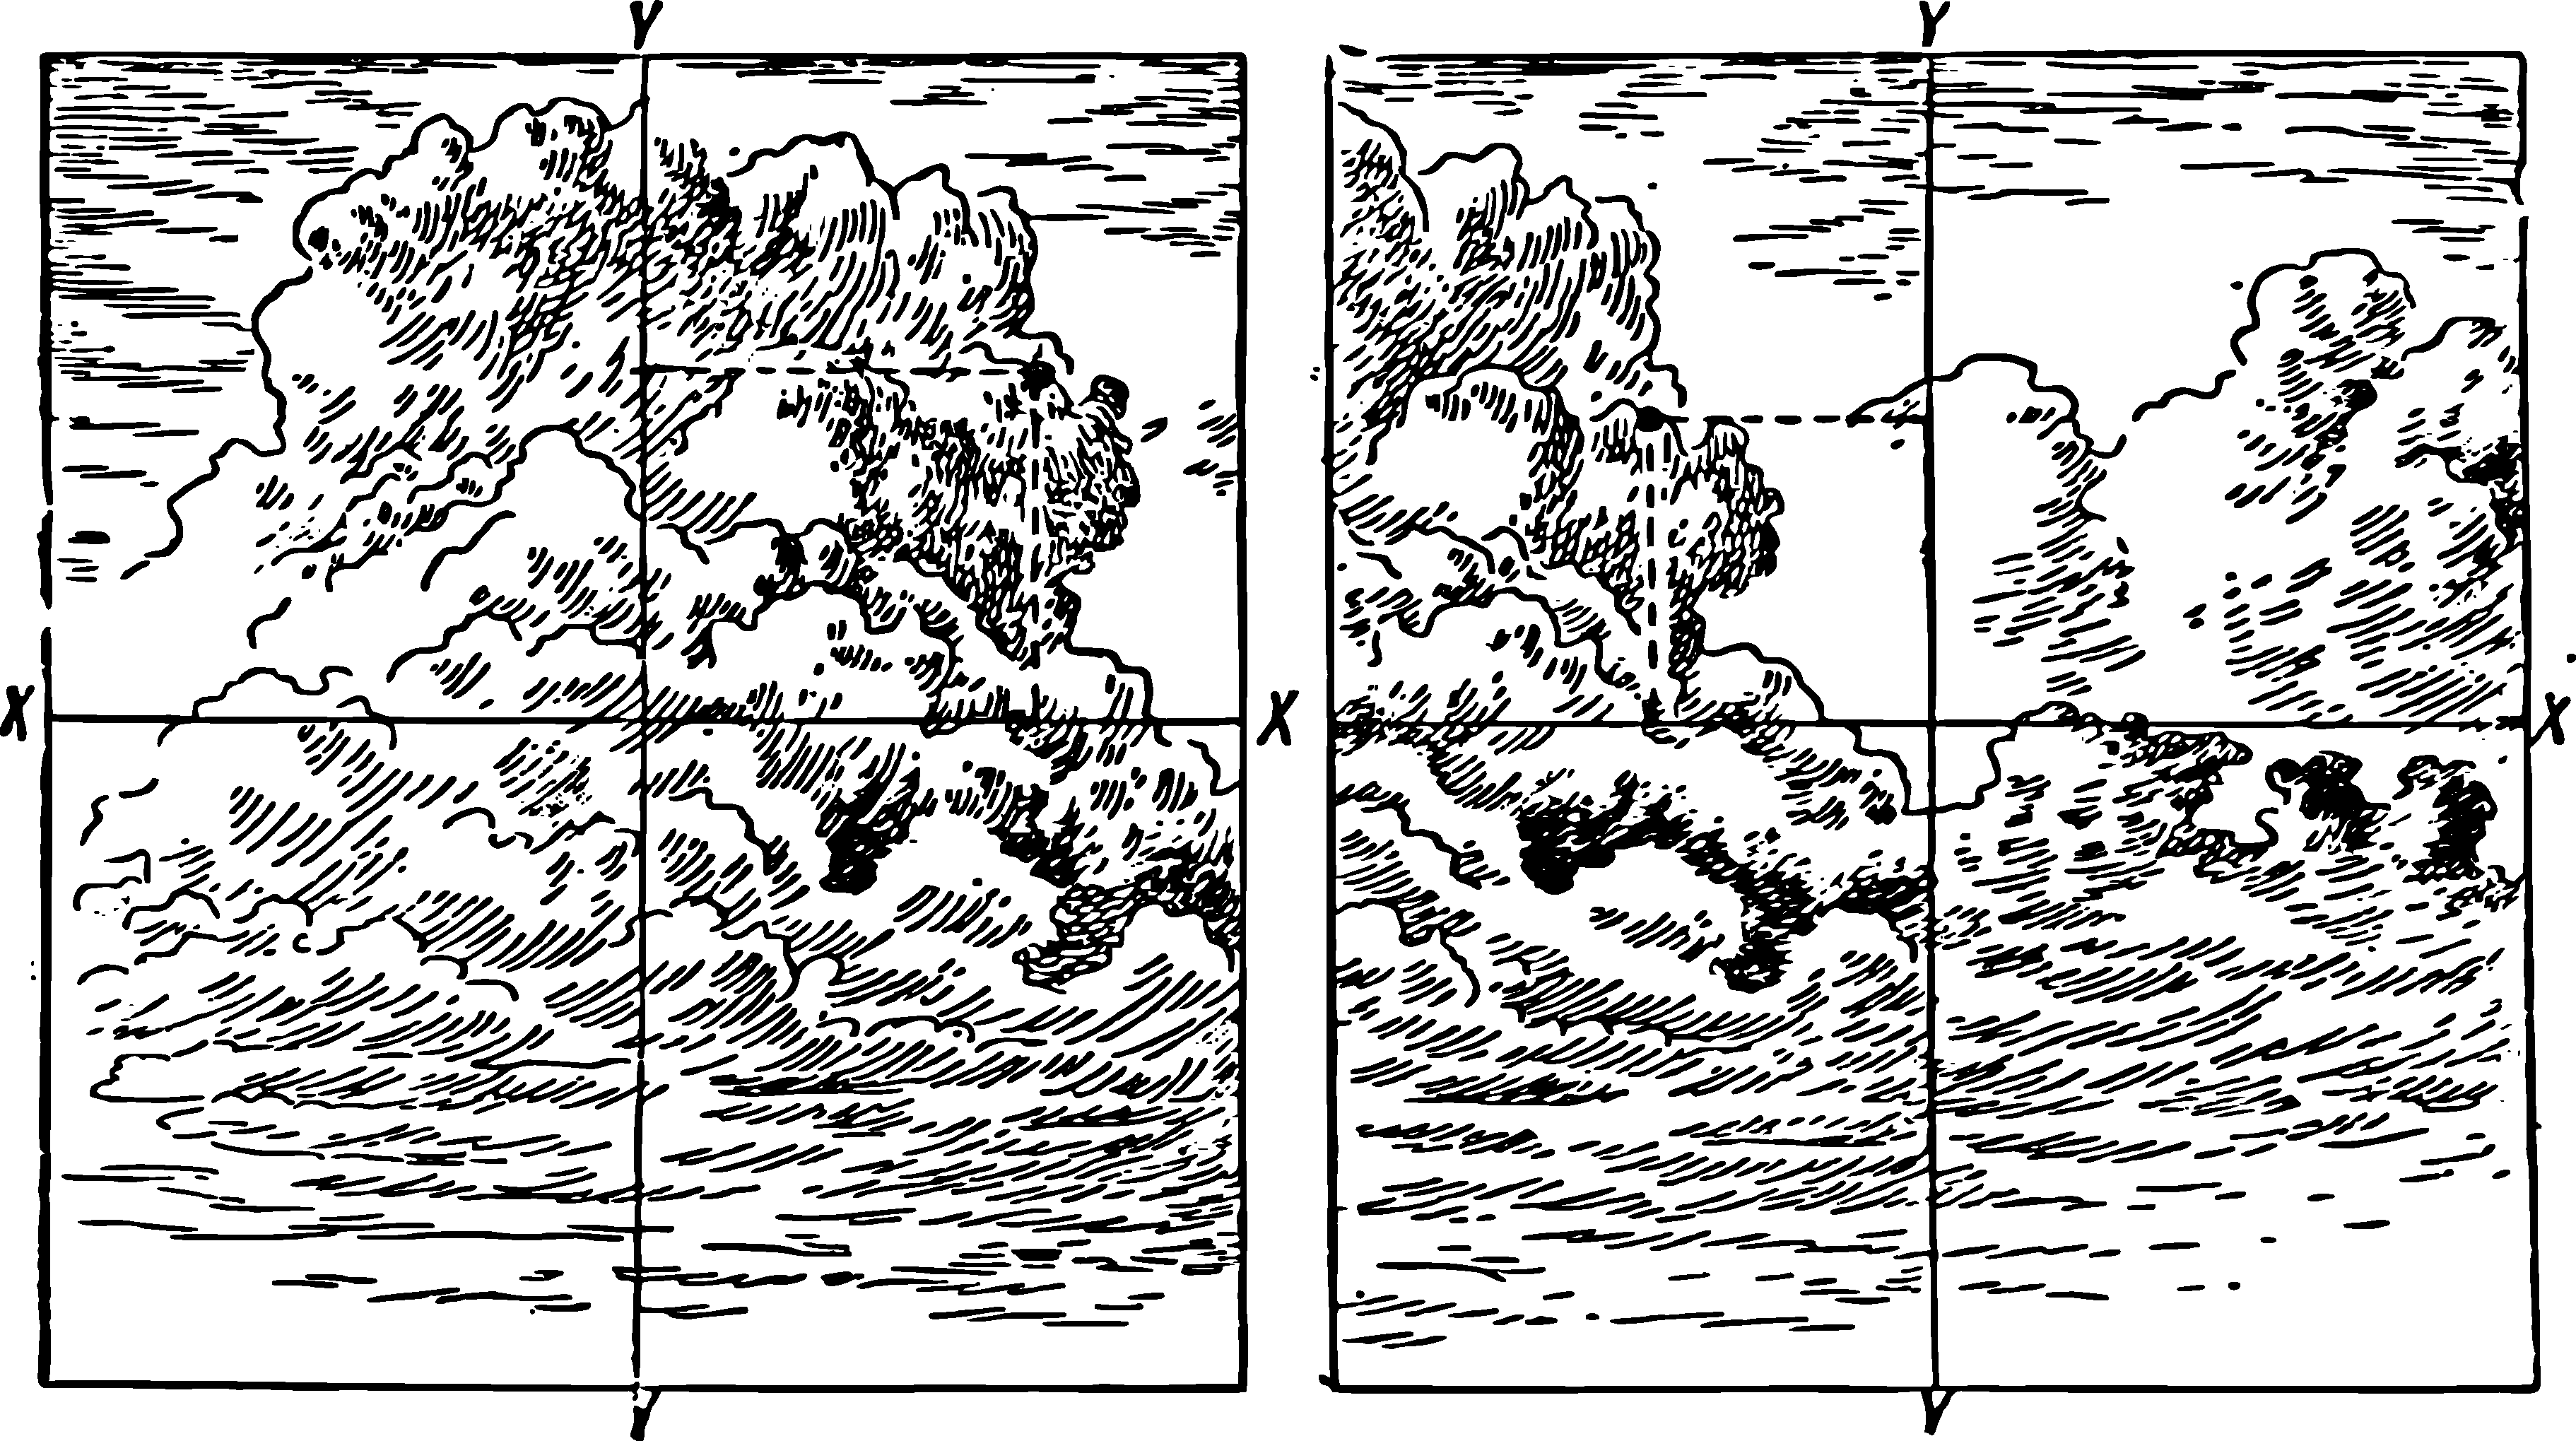
\includegraphics[width=\textwidth]{figures/ch-03/fig-076.pdf}
\sidecaption{An image of two photo prints of the cloud.\label{fig-076}}
\end{figure}

On the prints, which in size should be exactly equal to the photographic plates, they draw straight lines $YY$ and $XX$, connecting the midpoints of the opposite edges of the pictures (\figr{fig-076}). Then they mark on each picture the same point of the cloud and calculate its distances (in pixels) from the lines $YY$ and $XX$. These distances are denoted respectively by the letters $x_{1}$, $y_{1}$ for one picture and $x_{2}$, $y_{2}$ for the other.

If the marked points on the pictures turn out to be on different sides of the line $YY$ (as in \figr{fig-076}), then the height of the cloud $H$ is calculated by the formula
\begin{equation*}%
H = b \cdot \frac{F}{x_{1} + x_{2}},
\end{equation*}	
where $b$ is the length of the base (in \si{\meter}), $F$ is the focal length (in \si{\milli\meter}).

If the marked points turn out to be on the same side of the line$YY$, then the height of the cloud is determined by the formula
\begin{equation*}%
H = b \cdot \frac{F}{x_{1} - x_{2}}
\end{equation*}	
As for the distances $y_{1}$ and $y_{2}$, they are not needed to calculate $H$, but by comparing them with each other, one can determine the correctness of the shooting.

If the plates lay in the cassettes tightly and symmetrically, then y₁ will be equal to y₂. In practise, however, they will, of course, be slightly different.

Let us say, for example, that the distances from the lines $YY$ and $XX$ to the marked point of the cloud on the \emph{original} photographs are as follows:
\begin{align*}%
x_{1} & = \SI{32}{\milli\meter},\quad  y_{1} = \SI{29}{\milli\meter},\\
x_{2} & = \SI{23}{\milli\meter},\quad  y_{y} = \SI{25}{\milli\meter}.
\end{align*}
The focal lengths of the lenses $F = \SI{135}{\milli\meter}$ and the distance between the cameras (base) $H = \SI{937}{\meter}$.\sidenote{According to the experience described in the book by N. F. Platonov, \emph{The application of mathematical analysis to solving practical problems.} In the article \emph{Cloud Height}, N. F. Platonov provides a derivation of the formula for calculating M, describes the possible installations of devices for photographing fbblack and gives a number of practical tips.} Photographs show that to determine the height of the cloud, it is necessary to use the formula
\begin{align*}%
H & = b \cdot \frac{F}{x_{1} + x_{2}},\\
& =  \SI{937}{\meter} \frac{135}{32 + 23}\\
& \approx \SI{2300}{\meter}
\end{align*}	
So, the cloud was at a height of about \SI{2.3}{\kilo\meter} from the ground.

Those who want to understand the derivation of the formula for determining the height of the cloud can use the diagram shown in \figr{fig-077}.

\begin{figure}[h!]
\centering
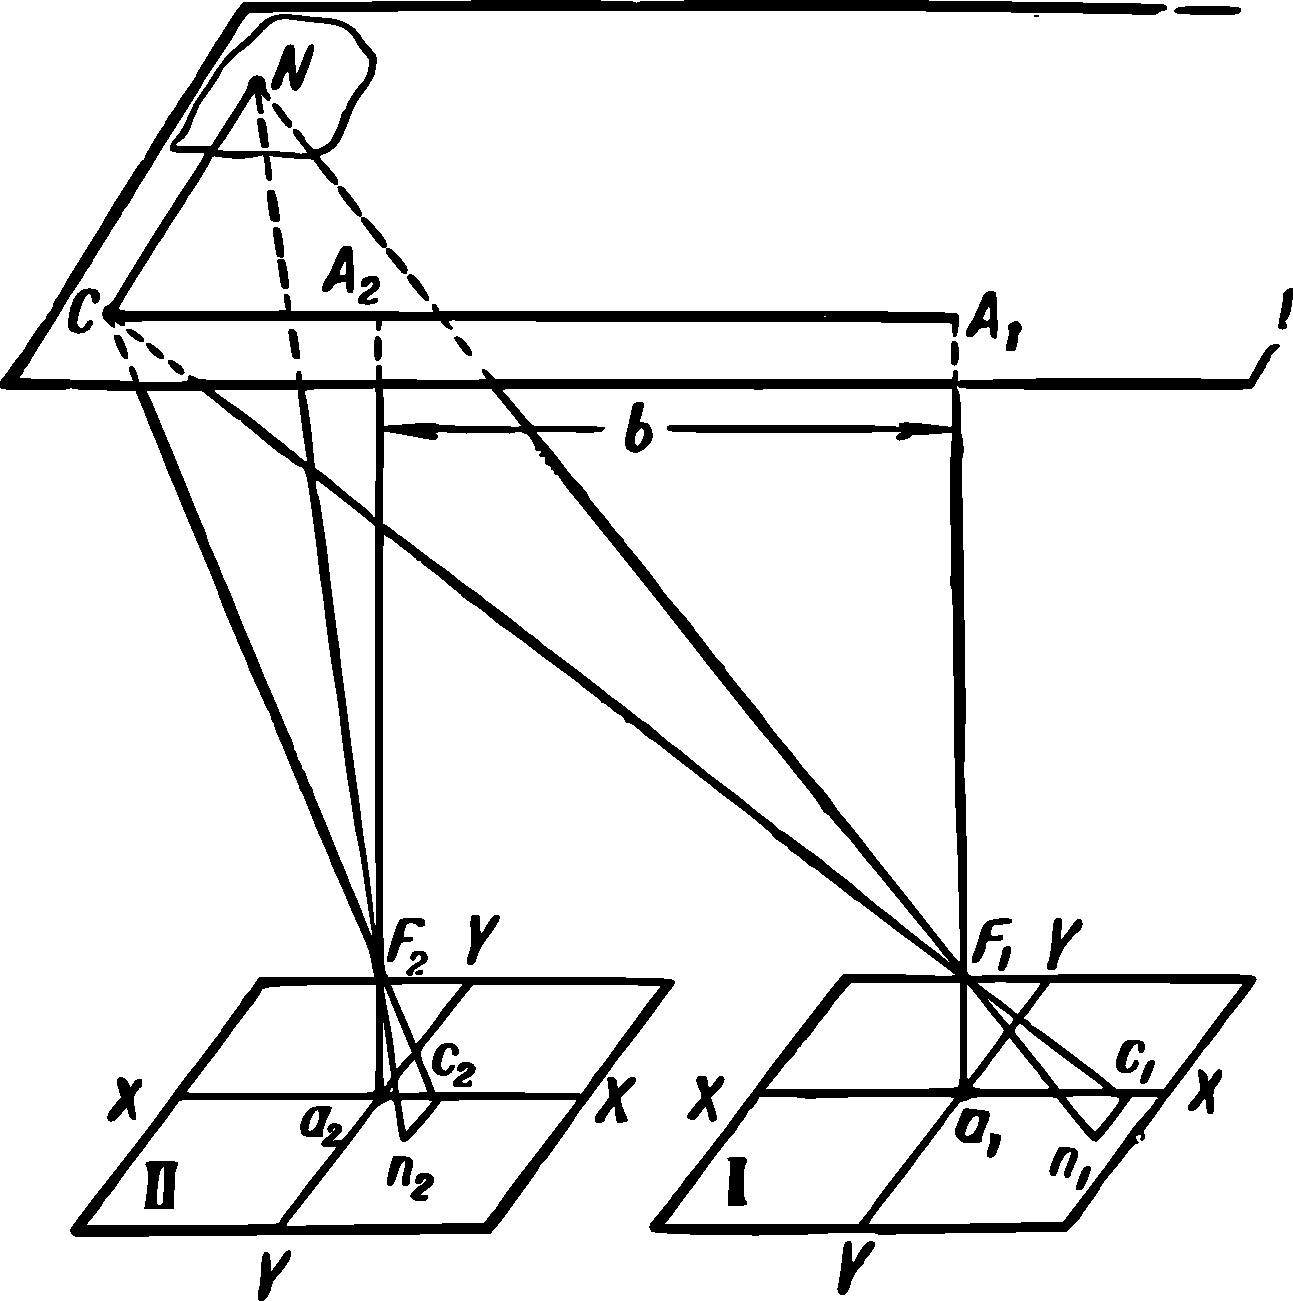
\includegraphics[width=0.8\textwidth]{figures/ch-03/fig-077.pdf}
\sidecaption{A diagram of the image of the cloud point on the plates of two cameras aimed at the zenith.\label{fig-077}}
\end{figure}

The drawing shown in \figr{fig-077} must be imagined in space (spatial imagination is developed in the study of that part of geometry called \emph{stereometry}).


Figures $I$ and $II$ -- images of photographic plates; $F_{1}$ and $F_{2}$ - optical centres of camera lenses; $N$ - observed point of the cloud; $n_{1}$ and $n_{2}$ -- images of point $N$ on the photographic plates; $a_{1}A_{1}$, and $a_{2}A_{2}$ -- perpendiculars raised from the midpoint of each photographic plate to the level of the cloud; $A_{1}A_{2} = a_{1}a_{2} = b$ the size of the baseline.

If we move from the optical centre $F_{1}$ upwards to point $A_{1}$, then from point $A_{1}$ along the baseline to such a point $C$ that will be the vertex of a right angle $A_{1}CN$, and finally, from point $C$ to point $N$, then segments $F_{1}A_{1}$, $A_{1}C_{1}$, and $CN$ in the camera will correspond to segments $F_{1}a_{1} = F$ (focal length), $a_{1}c_{1} = x_{1}$ and $c_{1}n_{1} = y_{1}$.

Similar constructions are used for the second camera. The proportions follow from the similarity of triangles
\begin{align*}%
\frac{A_{1}C}{x_{1}} & = \frac{A_{1}F_{1}}{F} = \frac{C_{1}F_{1}}{F_{1}c} = \frac{CN}{y_{1}} \qand \\
\frac{A_{2}C}{x_{2}} & = \frac{A_{2}F_{2}}{F} = \frac{C_{2}F_{2}}{F_{2}c} = \frac{CN}{y_{2}}.
\end{align*}
Comparing these proportions and bearing in mind the obvious equality of $A_{2}F_{2} = A_{1}F_{1}$, we find, firstly, that $y_{1} = y_{2}$ (a sign of correct shooting), secondly, that
\begin{equation*}%
\frac{A_{1}C}{x_{1}} = \frac{A_{2}C}{x_{2}};
\end{equation*}	
according to the drawing $A_{2}C = A_{1}C - b$, therefore,
\begin{align*}%
\frac{A_{1}C}{x_{1}} & = \frac{A_{1}C - b_{1}}{x_{2}}; \qor \\
A_{1}C & = b \cdot \frac{x_{1}}{x_{1} - x_{2}}, \text{finally},\\
A_{1}F_{1} & \approx  H = b \cdot \frac{F}{x_{1} - x_{2}}.
\end{align*}	
If $n_{1}$ and $n_{2}$--— the images on the plates of point $N$ — turned out to be on different sides of the straight line, this would indicate that point $C$ is between points $A_{1}$ and $A_{2}$, and then $A_{2}C = b - A_{1}C$, and the desired height
\begin{equation*}%
 H = b \cdot \frac{F}{x_{1} + x_{2}}.
\end{equation*}
These formulas apply only to the case when the optical axes of the cameras are aimed at the zenith. If the cloud is far from the zenith and near the horizon? If the vision of the devices does not fall, then you can give the devices a different position (while maintaining the parallelism of the optical axes), for example, direct them horizontally and, moreover, perpendicular to the basis or along the basis. 

For each position of the devices, it is necessary to first build an appropriate drawing and derive formulas for determining the height of the cloud.

\ques Here, ``in broad daylight'', noticeable feathery, highly layered clouds appeared in the sky of a whitish colour. Determine their height two or three times at certain intervals. If it turns out that the clouds have descended, this is a sign of worsening weather: expect rain in a few hours.

Take a picture of a floating balloon or stratostat and determine its height.

Here's the translation of the text:

---

\section{Tower Height from Photograph}

\ques Using a camera, one can determine not only the height of a cloud or a flying airplane but also the height of a ground structure: towers, masts, antennas, etc.

In \figr{fig-078} -- a photograph of the wind turbine of the Central Wind Turbine Institute (TSVEI), installed in Crimea near Balaklava. At the base of the tower is a square, the side length of which, let's assume, you know as a result of direct measurement: 6 meters.

\begin{figure}[h!]
\centering
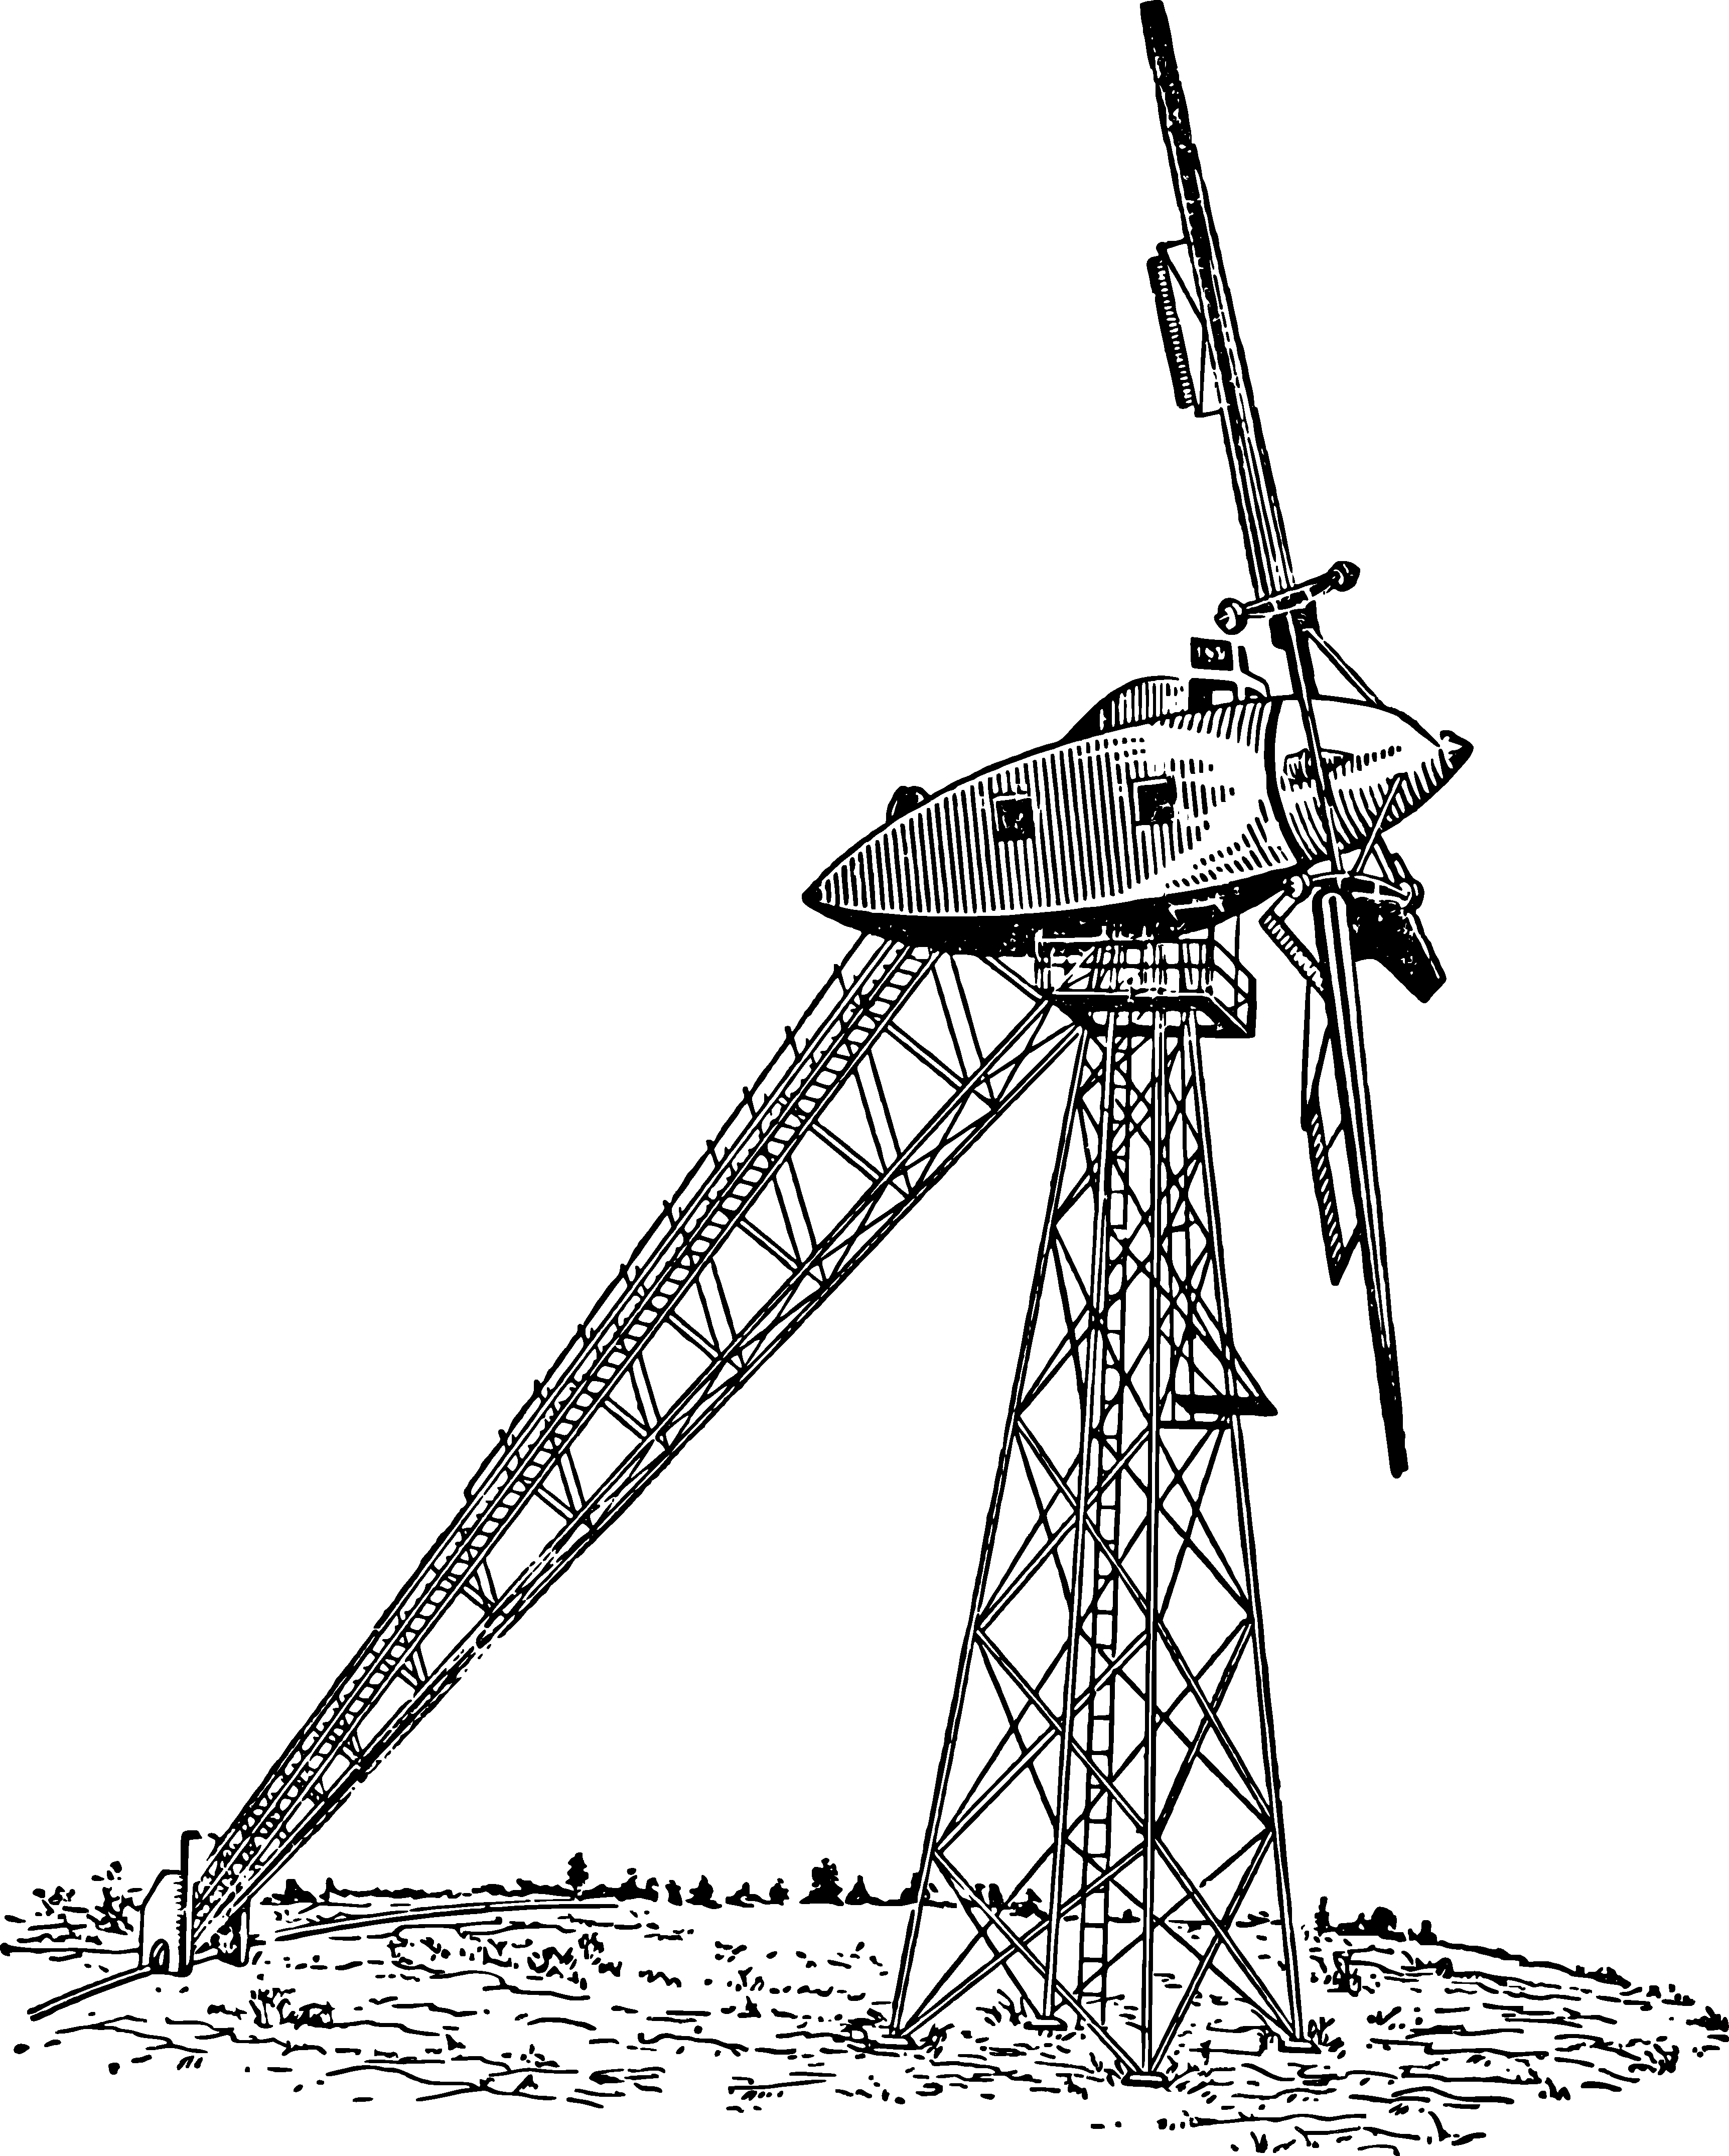
\includegraphics[width=0.8\textwidth]{figures/ch-03/fig-078.pdf}
\sidecaption{The wind turbine of the Central Wind Turbine Institute  in Crimea.\label{fig-078}}
\end{figure}

Make the necessary measurements on the photograph and determine the height of the entire wind turbine installation.


\ans The photograph of the tower and its true outline are geometrically similar to each other. Therefore, the height of the tower in real life is as many times greater than the height of its image as the image of the height is greater than the image of the base.

Measurements of the image: the length of the least distorted diagonal of the base is \SI{23}{\milli\meter}, the height of the entire installation is \SI{71}{\milli\meter}.

Since the length of the side of the square base of the tower is \SI{6}{\meter}, the diagonal of the base is $6^{2} + 6^{2} = 6\sqrt{2} \approx \SI{8.48}{\meter}$. Therefore, 
\begin{align*}%
\frac{71}{23} & = \frac{h}{8.48},\,\, \text{then}\\
h & = \frac{71 \times 8.48}{23} \approx \SI{26}{\meter}.
\end{align*}
Of course, not every photograph is suitable; only one in which the proportions are not distorted, as can happen with inexperienced photographers.


\section{Exercises}

Let the reader now apply the information gleaned from this chapter to solve a series of diverse problems:
\begin{enumerate}
\item A person of average height (1.7 m) is seen from a distance at an angle of \ang{;12}. Find the distance to him.

\item A cavalryman on horseback (2.2 m) is seen from a distance at an angle of \ang{;9}. Find the distance to him.

\item A telegraph pole (8 m) is seen at an angle of \ang{;22}. Find the distance to it.

\item A lighthouse with a height of 42 m is visible from a ship at an angle of \ang{1;10}. At what distance from the lighthouse is the ship?

\item The Earth is observed from the Moon at an angle of \ang{1;54}. Determine the distance from the Moon to the Earth.

\item A building is visible from a distance of 2 km at an angle of \ang{;12}. Find the height of the building.

\item The Moon is visible from the Earth at an angle of \ang{;30}. Knowing that the distance to the Moon is 380,000 km, determine its diameter.

\item How large should the letters on the classroom board be so that students sitting at their desks see them as clearly as the letters in their books (at a distance of 25 cm from the eye)? Take the distance from the desks to the board as 5 m.

\item A microscope magnifies 50 times. Can it be used to observe human blood cells, the diameter of which is 0.007 mm?

\item If there were people on the Moon of our height, what magnification of a telescope would be required to distinguish them from Earth?

\item How many `thousandths' are there in one degree?

\item How many degrees are there in one `thousandth'?

13. An airplane, moving perpendicular to the line of our observation, travels a distance visible at an angle of 300 `thousandths' in 10 seconds. Determine the speed of the airplane if the distance to it is 2000 m?

\end{enumerate}
\begin{center}
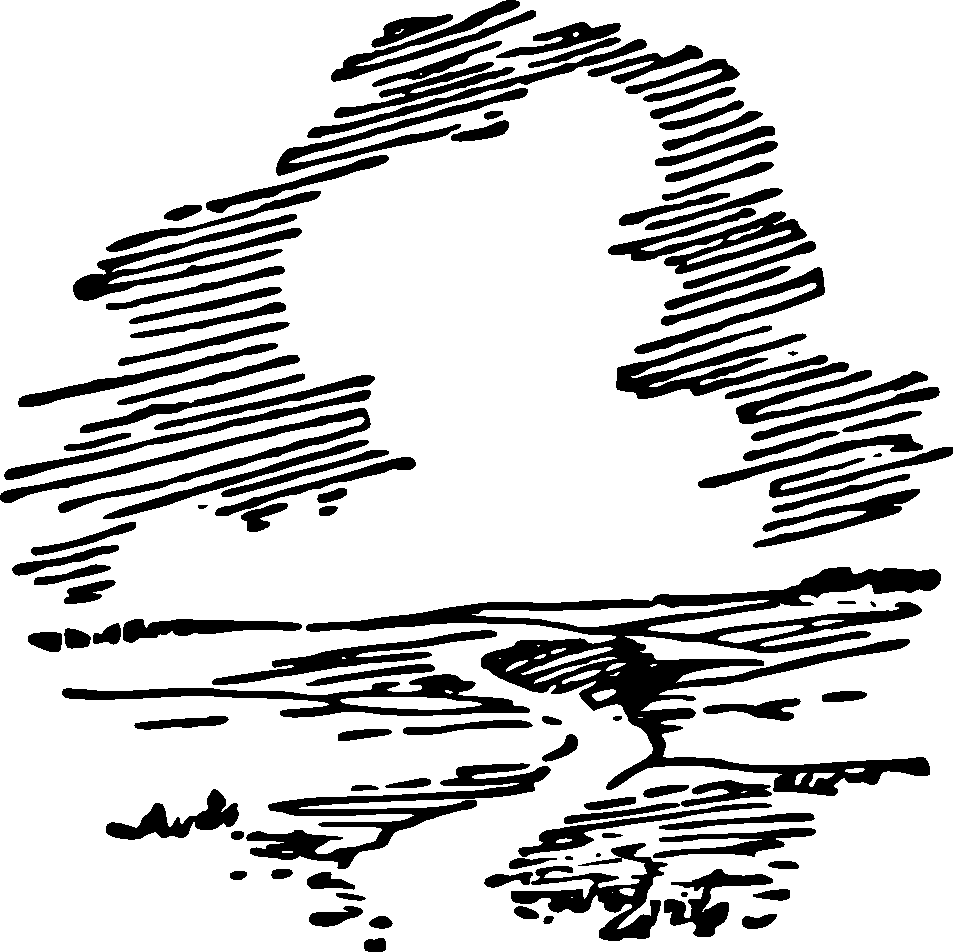
\includegraphics[width=0.3\textwidth]{figures/ch-03/fig-ch-03-tail.pdf}
\end{center}


















